%%%%%%%%%%%%%%%%%%%%%%%%%%%%%%%%%%%%%%%%%
% kaobook
% LaTeX Template
% Version 1.3 (December 9, 2021)
%
% This template originates from:
% https://www.LaTeXTemplates.com
%
% For the latest template development version and to make contributions:
% https://github.com/fmarotta/kaobook
%
% Authors:
% Federico Marotta (federicomarotta@mail.com)
% Based on the doctoral thesis of Ken Arroyo Ohori (https://3d.bk.tudelft.nl/ken/en)
% and on the Tufte-LaTeX class.
% Modified for LaTeX Templates by Vel (vel@latextemplates.com)
%
% License:
% CC0 1.0 Universal (see included MANIFEST.md file)
%
%%%%%%%%%%%%%%%%%%%%%%%%%%%%%%%%%%%%%%%%%

%----------------------------------------------------------------------------------------
%	PACKAGES AND OTHER DOCUMENT CONFIGURATIONS
%----------------------------------------------------------------------------------------

\documentclass[
	a4paper, % Page size
	fontsize=10pt, % Base font size
	twoside=true, % Use different layouts for even and odd pages (in particular, if twoside=true, the margin column will be always on the outside)
	%open=any, % If twoside=true, uncomment this to force new chapters to start on any page, not only on right (odd) pages
	%chapterentrydots=true, % Uncomment to output dots from the chapter name to the page number in the table of contents
	numbers=noenddot, % Comment to output dots after chapter numbers; the most common values for this option are: enddot, noenddot and auto (see the KOMAScript documentation for an in-depth explanation)
]{kaobook}

% Choose the language
\ifxetexorluatex
	\usepackage{polyglossia}
	\setmainlanguage{english}
\else
	\usepackage[english]{babel} % Load characters and hyphenation
\fi
\usepackage{csquotes}	% English quotes
\usepackage{epigraph}	% English quotes

% Load packages for testing
\usepackage{blindtext}
% \usepackage{showframe} % Uncomment to show boxes around the text area, margin, header and footer
%\usepackage{showlabels} % Uncomment to output the content of \label commands to the document where they are used

% Load the bibliography package
\usepackage{kaobiblio}
\addbibresource{main.bib} % Bibliography file

% Load mathematical packages for theorems and related environments
\usepackage[framed=true]{kaotheorems}

% Load the package for hyperreferences
\usepackage{kaorefs}

\graphicspath{{examples/documentation/images/}{images/}} % Paths in which to look for images

\makeindex[columns=3, title=Alphabetical Index, intoc] % Make LaTeX produce the files required to compile the index

\makeglossaries % Make LaTeX produce the files required to compile the glossary
\newglossaryentry{computer}{
	name=computer,
	description={is a programmable machine that receives input, stores and manipulates data, and provides output in a useful format}
}

% Glossary entries (used in text with e.g. \acrfull{fpsLabel} or \acrshort{fpsLabel})
\newacronym[longplural={Frames per Second}]{fpsLabel}{FPS}{Frame per Second}
\newacronym[longplural={Tables of Contents}]{tocLabel}{TOC}{Table of Contents}

 % Include the glossary definitions

\makenomenclature % Make LaTeX produce the files required to compile the nomenclature

% Reset sidenote counter at chapters
%\counterwithin*{sidenote}{chapter}

\usepackage{needspace}
\usetikzlibrary{positioning}
%----------------------------------------------------------------------------------------

\begin{document}

%----------------------------------------------------------------------------------------
%	BOOK INFORMATION
%----------------------------------------------------------------------------------------

% \titlehead{The \texttt{kaobook} class}
% \subject{Use this document as a template}

% \title[Example and documentation of the {\normalfont\texttt{kaobook}} class]{Example and documentation \\ of the {\normalfont\texttt{kaobook}} class}
\title{Navigating Linux System Commands}
\subtitle{A guide for beginners to the Linux Shell and GNU coreutils}

\author{Sayan Ghosh}

\date{\today}

\publishers{IIT Madras \\ BS Data Science and Applications}

%----------------------------------------------------------------------------------------

\frontmatter % Denotes the start of the pre-document content, uses roman numerals

%----------------------------------------------------------------------------------------
%	OPENING PAGE
%----------------------------------------------------------------------------------------

% \makeatletter
% \extratitle{
% % In the title page, the title is vspaced by 9.5\baselineskip
% \vspace*{9\baselineskip}
% \vspace*{\parskip}
% \begin{center}
% 	% In the title page, \huge is set after the komafont for title
% 	\usekomafont{title}\Huge\@title
% \end{center}
% }
% \makeatother

%----------------------------------------------------------------------------------------
%	COPYRIGHT PAGE
%----------------------------------------------------------------------------------------

\makeatletter
\uppertitleback{\@titlehead} % Header

\lowertitleback{
	\textbf{Disclaimer}\\
	This document is a companion activity book
  for the System Commands (BSSE2001) course taught by
  \textbf{
    \href{https://home.iitm.ac.in/gphani/}{Prof. Gandham Phanikumar}
    }
    at
    \textbf{
      \href{https://study.iitm.ac.in/ds/}{IIT Madras BS Program}.
      }
      This book contains resources, references, questions and solutions to some
      common questions on Linux commands, shell scripting,
      grep, sed, awk, and other system commands. \\ \\
      This was prepared with the help and guidance of the course instructors: \\
      \begin{center}
        \textbf{
          Santhana Krishnan
          } and
          \textbf{
            Sushil Pachpinde
            }
      \end{center}

	    \medskip

	    \textbf{Copyright}\\
	    \copyright\
      This book is released under the public domain, meaning it is freely available for use and distribution without restriction. However, while the content itself is not subject to copyright, it is requested that proper attribution be given if any part of this book is quoted or referenced. This ensures recognition of the original authorship and helps maintain transparency in the dissemination of information.

	\medskip

	\textbf{Colophon} \\
	This document was typeset with the help of \href{https://sourceforge.net/projects/koma-script/}{\KOMAScript} and \href{https://www.latex-project.org/}{\LaTeX} using the \href{https://github.com/fmarotta/kaobook/}{kaobook} class.

	The source code of this book is available at:\\\url{https://github.com/sayan01/se2001-book}

	(You are welcome to contribute!)

	\medskip

	\textbf{Edition} \\
	Compiled on \today
}
\makeatother

%----------------------------------------------------------------------------------------
%	DEDICATION
%----------------------------------------------------------------------------------------

\dedication{
UNIX is basically a simple operating
system, but you have to be a genius
to understand the simplicity.\\
	\flushright -- Dennis Ritchie
}

%----------------------------------------------------------------------------------------
%	OUTPUT TITLE PAGE AND PREVIOUS
%----------------------------------------------------------------------------------------

% Note that \maketitle outputs the pages before here

\maketitle

%----------------------------------------------------------------------------------------
%	PREFACE
%----------------------------------------------------------------------------------------

\chapter*{Preface}
\addcontentsline{toc}{chapter}{Preface} % Add the preface to the table of contents as a chapter

Through this work I have tried to make learning and
understanding the basics of Linux fun and easy. I have
tried to make the book as practical as possible, with
many examples and exercises. The structure of the book
follows the structure of the course \textit{BSSE2001
- System Commands}, taught by
\textbf{
\href{https://home.iitm.ac.in/gphani/}{Prof. Gandham Phanikumar}
}
at
\textbf{
\href{https://study.iitm.ac.in/ds/}{IIT Madras BS Program}.
}.

The book takes inspiration from the previous works done for the course,

\begin{itemize}
	\item \href{https://github.com/prassr}{Sanjay Kumar}'s
	\href{https://github.com/prassr/gnu-linux-commands}{Github Repository}
	\item \href{https://github.com/cheriangeorge}{Cherian George}'s
	\href{https://github.com/prassr/gnu-linux-commands}{Github Repository}
	\item \href{https://github.com/prabuddhmathur}{Prabuddh Mathur}'s
	\href{https://www.youtube.com/playlist?list=PLLuZiiAWg2wpaEOBWAVO7Jl35MQkOyi6-}{TA Sessions}
\end{itemize}

as well as external resources like:

\begin{itemize}
	\item \href{https://www.robertelder.org/}{Robert Elder}'s
	\href{https://blog.robertelder.org/}{Blogs} and
	\href{https://www.youtube.com/@RobertElderSoftware/shorts}{Videos}
	\item \href{https://www.aalto.fi/en}{Aalto University, Finland}'s
	\href{https://scicomp.aalto.fi/scicomp/shell/}{Scientific Computing - Linux Shell Crash Course}
\end{itemize}

The book covers basic commands, their motivation, use cases, and examples.
The book also covers some advanced topics like shell scripting, regular expressions, and text processing using \texttt{sed} and \texttt{awk}.

This is not a substitute for the course, but a companion to it.
The book is a work in progress and any contribution is welcome at
\url{https://github.com/sayan01/se2001-book}

\begin{flushright}
	\textit{Sayan Ghosh}
\end{flushright}

\index{preface}

%----------------------------------------------------------------------------------------
%	TABLE OF CONTENTS & LIST OF FIGURES/TABLES
%----------------------------------------------------------------------------------------

\begingroup % Local scope for the following commands

% Define the style for the TOC, LOF, and LOT
%\setstretch{1} % Uncomment to modify line spacing in the ToC
%\hypersetup{linkcolor=blue} % Uncomment to set the colour of links in the ToC
\setlength{\textheight}{230\hscale} % Manually adjust the height of the ToC pages

% Turn on compatibility mode for the etoc package
\etocstandarddisplaystyle % "toc display" as if etoc was not loaded
\etocstandardlines % "toc lines" as if etoc was not loaded

\tableofcontents % Output the table of contents

\listoffigures % Output the list of figures

% Comment both of the following lines to have the LOF and the LOT on different pages
\let\cleardoublepage\bigskip
\let\clearpage\bigskip

\listoftables % Output the list of tables

\endgroup

%----------------------------------------------------------------------------------------
%	MAIN BODY
%----------------------------------------------------------------------------------------

\mainmatter % Denotes the start of the main document content, resets page numbering and uses arabic numbers
\setchapterstyle{kao} % Choose the default chapter heading style

\setchapterpreamble[u]{\margintoc}
\chapter{Basic Commands in Linux}
\labch{basic}

\section{Navigating the File System}
The file system can be navigated in the Linux command line using the following commands:
\begin{itemize}
  \item \textbf{pwd}: Print the current working directory
  \item \textbf{ls}: List the contents of the current directory
  \item \textbf{cd}: Change the current working directory
  \item \textbf{mkdir}: Create a new directory
  \item \textbf{rmdir}: Remove a directory
  \item \textbf{touch}: Create a new file
  \item \textbf{rm}: Remove a file
  \item \textbf{pushd}: Push the current directory to a stack
  \item \textbf{popd}: Pop the current directory from a stack\sidenote{\textbf{pushd} and \textbf{popd} are useful for quickly switching between directories in scripts.}
\end{itemize}

More details about these commands can be found in their respective
man pages. For example, to find more about the \textbf{ls} command,
you can type \texttt{man ls}

\begin{qs}
  What is the command to list the contents of the current directory?
\end{qs}

\begin{ans}
  \texttt{ls}
\end{ans}


\begin{qs}
  What is the command to list the contents of the current directory
  including hidden files?
\end{qs}

\begin{ans}
\texttt{ls -a}
\end{ans}

\begin{qs}
  What is the command to list the contents of the current directory
  in a long list format? (show permissions, owner, group, size, and time)
\end{qs}

\begin{ans}
\texttt{ls -l}
\end{ans}

\begin{qs}
  What is the command to list the contents of the current directory
  in a long list format and also show hidden files?
\end{qs}

\begin{ans}
\texttt{ls -al} or \texttt{ls -la} or \texttt{ls -l -a} or \texttt{ls -a -l}
\end{ans}

\begin{qs}
  The output of \texttt{ls} gives multiple files and directories in a single
  line. How can you make it print one file or directory per line?
\end{qs}

\begin{ans}
  \texttt{ls -1}\\
  This can also be done by passing the output of \texttt{ls} to \texttt{cat}
  or storing the output of \texttt{ls} in a file and then using \texttt{cat}
  to print it. We will see these in later weeks.\sidenote{that is a one, not an L}
\end{ans}

\section{File Permissions}
\begin{qs}
  How to list the permissions of a file?
\end{qs}

\begin{ans}
  \texttt{ls -l} \\
  The permissions are the first 10 characters of the output.\\
  \texttt{stat -c \%A filename} will list only the permissions of a file.\\
  There are other format specifiers of \texttt{stat} to show different statistics
  which can be found in \texttt{man stat}.
\end{ans}

\begin{qs}
  How to change permissions of a file?
  Let's say we want to change \texttt{file1}'s permissions to \texttt{rwxr-xr--}
  What is the octal form of that?
\end{qs}

\begin{ans}
  \texttt{chmod u=rwx,g=rx,o=r file1} will change the permissions of \texttt{file1}\\
  The octal form of \texttt{rwxr-xr--} is 754.\\
  So we can also use \texttt{chmod 754 file1}\\
  Providing the octal is same as using \texttt{=} to set the permissions.\\
  We can also use \texttt{+} to add permissions and \texttt{-} to remove permissions.
\end{ans}

\section{Inodes and Links}

\begin{qs}
  How to list the inodes of a file?
\end{qs}

\begin{ans}
  \texttt{ls -i} will list the inodes of a file.
  The inodes are the first column of the output of \texttt{ls -i}
  This can be combined with other flags like \texttt{-l} or \texttt{-a} to show more details.
\end{ans}

\begin{qs}
  How to create soft link of a file?
\end{qs}

\begin{ans}
  \texttt{ln -s sourcefile targetfile} will create a soft link of \texttt{sourcefile}
  named \texttt{targetfile}.
  The soft link is a pointer to the original file.
\end{ans}

\begin{definition}[Soft Links]
\labdef{softlinks}
  Soft Links are special kinds of files that just store the path
  given to them. Thus the path given while making soft links should
  either be an absolute path, or relative \textbf{from} the location of the
  soft link \textbf{to} the location of the original file. It should not be
  relative from current working directory.\footnote{This is a common mistake.}
\end{definition}

\begin{qs}
  How to create hard link of a file?
\end{qs}

\begin{ans}
  \texttt{ln sourcefile targetfile} will create a hard link of \texttt{sourcefile}
  named \texttt{targetfile}. The hard link is same as the original file. It does
  not depend on the original file anymore after creation. They are equals,
  both are \texttt{hardlinks} of each other. There is no parent-child relationship.
  The other file can be deleted and the original file will still work.
\end{ans}

\begin{definition}[Hard Links]
  Hard Links are just pointers to the same inode. They are the same file.
  They are not pointers to the path of the file. They are pointers to the
  file itself. They are not affected by the deletion of the other file.
  When creating a hard link, you need to provide the path of the original
  file, and thus it has to be either absolute path, or relative from the
  current working directory, not relative from the location of the hard link.
\end{definition}

\begin{qs}
  How to get the real path of a file?\\
  Assume three files:
  \begin{itemize}
    \item \textbf{file1} is a soft link to \textbf{file2}
    \item \textbf{file2} is a soft link to \textbf{file3}
    \item \textbf{file3} is a regular file
  \end{itemize}
  Real path of all these three should be the same. How to get that?
\end{qs}

\begin{ans}
  \texttt{realpath filename} will give the real path of \texttt{filename}. \\
  You can also use \texttt{readlink -f filename} to get the real path.
\end{ans}

\section{System Management and Information}

\begin{qs}
  How to print the current date and time in some custom format?
\end{qs}

\begin{ans}
  \texttt{date -d today +\%Y-\%m-\%d} will print the current date in the format
  \texttt{YYYY-MM-DD}. The format can be changed by changing the format specifiers.
  The format specifiers are given in the \texttt{man date} page. The \texttt{-d today} can
  be dropped, but is mentioned to show that the date can be changed to any date.
  It can be strings like '2024-01-01' or '5 days ago' or 'yesterday', etc.
\end{ans}

\begin{qs}
  How to print the kernel version of your system?
\end{qs}

\begin{ans}
  \texttt{uname -r} will print the kernel version of your system.
  \texttt{uname} is a command to print system information.
  The \texttt{-r} flag is to print the kernel release.
  There are other flags to print other system information. \\
  We can also run \texttt{uname -a} to get all fields and extract only the
  kernel info using commands taught in later weeks.
\end{ans}

\begin{qs}
  How to see how long your system is running for? \\
  What about the time it was booted up?
\end{qs}

\begin{ans}
  \texttt{uptime} will show how long the system is running for.\\
  \texttt{uptime -s} will show the time the system was booted up. \\
  The \texttt{-s} flag is to show the time of last boot.
\end{ans}

\begin{qs}
  How to see the amount of free memory? What about free hard disk space?
  If we are unable to understand the big numbers, how to convert them to human readable format?
  What is difference between MB and MiB?
\end{qs}

\begin{ans}
  \texttt{free} will show the amount of free memory. \\
  \texttt{df} will show the amount of free hard disk space. \\
  \texttt{df -h} and \texttt{free -h}
  will convert the numbers to human readable format. \\
  MB is Megabyte, and MiB is Mebibyte. \\
  1 MB = 1000 KB, 1 GB = 1000 MB, 1 TB = 1000 GB, this is SI unit. \\
  1 MiB = 1024 KiB, 1 GiB = 1024 MiB, 1 TiB = 1024 GiB, this is $2^{10}$ unit.
\end{ans}

\section{Reading and Writing Files using cat}

\begin{qs}
  Can we print contents of multiple files using a single command?
\end{qs}

\begin{ans}
  \texttt{cat file1 file2 file3} will print the contents of \texttt{file1}, \texttt{file2}, and \texttt{file3}
  in the order given. The contents of the files will be printed one after the other.
\end{ans}

\begin{qs}
  Can \texttt{cat} also be used to write to a file?
\end{qs}

\begin{ans}
  Yes, \texttt{cat > file1} will write to \texttt{file1}. The input will be taken from the
  terminal and written to \texttt{file1}. The input will be written to \texttt{file1} until
  the user presses \texttt{Ctrl+D} to indicate end of input.
  This is \texttt{redirection}, which we see in later weeks.
\end{ans}

\begin{qs}
  \texttt{ls} can only show files and directories in the \textbf{cwd}\sidenote{\textbf{cwd} means \textbf{Current Working Directory}}, not subdirectories.
  True or False?
\end{qs}

\begin{ans}
  False. \texttt{ls} can show files and directories in the cwd, and also in subdirectories.
  The \texttt{-R} flag can be used to show files and directories in subdirectories, recursively.
\end{ans}

\section{Types of Files}

\begin{qs}
  What types of files are possible in a linux file system?
\end{qs}

\begin{ans}
  There are 7 types of files in a linux file system:
  \begin{itemize}
    \item Regular Files (starts with \texttt{-})
    \item Directories (starts with \texttt{d})
    \item Symbolic Links (starts with \texttt{l})
    \item Character Devices (starts with \texttt{c})
    \item Block Devices (starts with \texttt{b})
    \item Named Pipes (starts with \texttt{|})
    \item Sockets (starts with \texttt{s})
  \end{itemize}
\end{ans}

\begin{qs}
  How to know what kind of file a file is? Can we determine using
  its extension? Can we determine using its contents? What does
  \textit{
  \href{https://developer.mozilla.org/en-US/docs/Web/HTTP/Basics_of_HTTP/MIME_types}{MIME} mean?
}
How to get that?
\end{qs}

\begin{ans}
  The \texttt{file} command can be used to determine the type of a file. \\
  The extension of a file does not determine its type. \\
  The contents of a file can be used to determine its type. \\
  MIME stands for Multipurpose Internet Mail Extensions. \\
  It is a standard that indicates the nature and format of a document. \\
  \texttt{file -i filename} will give the MIME type of \texttt{filename}.
\end{ans}
\section{Types of Commands}

\begin{qs}
  How to create aliases? How to make them permanent? How to unset them?
\end{qs}

\begin{ans}
  \texttt{alias name='command'} will create an alias. \\
  \texttt{unalias name} will unset the alias. \\
  To make them permanent, add the alias to the \texttt{$\sim$/.bashrc} file. \\
  The \texttt{$\sim$/.bashrc} file is a script that is executed whenever a new terminal is opened.
\end{ans}

\begin{qs}
  How to run the normal version of a command if it is aliased?
\end{qs}

\begin{ans}
  \texttt{\textbackslash command} will run the normal version of \texttt{command} if it is aliased.
\end{ans}

\begin{qs}
  What is the difference between \texttt{which}, \texttt{whatis}, \texttt{whereis}, \texttt{locate}, and \texttt{type}?
\end{qs}

\begin{ans}
  Each of the commands serve a different purpose:
  \begin{itemize}
    \item \texttt{which} will show the path of the command that will be executed.
    \item \texttt{whatis} will show a short description of the command.
    \item \texttt{whereis} will show the location of the command, source files, and man pages.
    \item \texttt{locate} is used to find files by name.
    \item \texttt{type} will show how the command will be interpreted by the shell.
  \end{itemize}
\end{ans}

\begin{exercise}
  Find the path of the \texttt{true} command using \texttt{which}.
  Find a short description of the \texttt{true} command using \texttt{whatis}.
  Is the executable you found actually the one that is executed when you run \texttt{true}? Check using \texttt{type true}
\end{exercise}

\begin{definition}[Types of commands]
  A command can be an alias, a shell built-in, a shell function, keyword, or an executable.
  The \texttt{type} command will show which type the command is.
  \begin{itemize}
    \item \textbf{alias}: A command that is an alias to another command defined
    by the user or the system.
    \item \textbf{builtin}: A shell built-in command is a command that is built
    into the shell itself. It is executed internally by the shell.
    \item \textbf{file}: An executable file that is stored in the file system.
      It has to be stored somewhere in the \textbf{PATH} variable.
    \item \textbf{function}: A shell function is a set of commands that are
    executed when the function is called.
    \item \textbf{keyword}: A keyword is a reserved word that is part of the shell
    syntax. It is not a command, but a part of the shell syntax.
  \end{itemize}
\end{definition}

\section{File Manipulation}

\begin{qs}
  How to list only first 10 lines of a file? How about first 5? Last 5?
  How about lines 105 to lines 152?
\end{qs}

\begin{ans}
  \texttt{head filename} will list the first 10 lines of \texttt{filename}. \\
  \texttt{head -n 5 filename} will list the first 5 lines of \texttt{filename}. \\
  \texttt{tail -n 5 filename} will list the last 5 lines of \texttt{filename}. \\
  \texttt{head -n 152 filename | tail -n 48} will list lines 105 to 152 of \texttt{filename}.
  This uses \texttt{|} which is a pipe, which we will see in later weeks.
\end{ans}

\begin{qs}
  Do you know how many lines a file contains? How can we count it?
  What about words? Characters?
\end{qs}

\begin{ans}
  \texttt{wc filename} will count the number of lines, words, and characters in \texttt{filename}. \\
  \texttt{wc -l filename} will count the number of lines in \texttt{filename}. \\
  \texttt{wc -w filename} will count the number of words in \texttt{filename}. \\
  \texttt{wc -c filename} will count the number of characters in \texttt{filename}.
\end{ans}

\begin{qs}
  How to delete an empty directory? What about non-empty directory?
\end{qs}

\begin{ans}
  \texttt{rmdir dirname} will delete an empty directory. \\
  \texttt{rm -r dirname} will delete a non-empty directory.
\end{ans}

\begin{qs}
  How to copy an entire folder to another name? What about moving? \\
  Why the difference in flags?
\end{qs}

\begin{ans}
  \texttt{cp -r sourcefolder targetfolder} will copy an entire folder to another name. \\
  \texttt{mv sourcefolder targetfolder} will move an entire folder to another name. \\
  The difference in flags is because \texttt{cp} is used to copy, and \texttt{mv} is used to move or rename a file or folder.
  The \texttt{-r} flag is to copy recursively, and is not needed for \texttt{mv} as it is not recursive
  and simply changes the name of the folder (or the path).
\end{ans}

% % \setchapterpreamble[u]{\margintoc}
\chapter{Shell Variables}
\labch{variables}

We have seen how to execute commands in the linux shell, and also how to
combine those commands to perform complex tasks. However, to make really
powerful scripts, we need to store the output of commands, and also store
intermediate results. This is where variables come in. In this chapter,
we will learn how to create, manipulate, and use variables in the shell.

\section{Creating Variables}

There are two types of variables in the shell: \textbf{Environment Variables}
and \textbf{Shell Variables}. Environment variables are accessible to all
processes running in the environment, while shell variables are only accessible
to the shell in which they are created.

\begin{definition}[Environment Variables]
  An environment variable is a variable that is accessbile to all
  processes running in the environment. It is a key-value pair.
  It is created using the \lstinline{export} command. It can be accessed
  using the \$ followed by the name of the variable (e.g. \$HOME) or
  using the \lstinline{printenv} command.
  They are part of the environment in which a process runs. 
  A running process can thus access the value of the environment variable
  HOME to find the home directory of the user running the process,
  or the PATH variable to find the directories to search for commands.
\end{definition}

\begin{definition}[Shell Variables]
  A shell variable is a variable that is only accessible to the shell
  in which it is created. It is a key-value pair. It is created using
  the \lstinline{=} operator. It can be accessed using the \$ followed by the name
  of the variable (e.g. \$var).
  They are local to the shell in which they are created.
\end{definition}

Let us see how to create a shell variable.

\begin{lstlisting}[language=bash]
$ var="Hello World"
\end{lstlisting}

This creates a shell variable \lstinline{var} with value \lstinline{Hello World}.
If the value of our variable contains spaces, we need to enclose it in quotes.

\begin{remark}
Note that there should be \textbf{no spaces} around the \lstinline{=} operator.
\end{remark}

Variable names can contain letters, numbers, and underscores, but they cannot start with a number.

Similarly, for an environment variable, we use the \lstinline{export} command.

\begin{lstlisting}[language=bash]
$ export var="Hello World"
\end{lstlisting}

This creates an environment variable \lstinline{var} with value \lstinline{Hello World}.
The difference between a shell variable and an environment variable is that the environment variable is accessible to all processes running in the environment, while the shell variable is only accessible to the shell in which it is created.

A variable can also be exported after it is created.

\begin{lstlisting}[language=bash]
$ var="Hello World"
$ export var
\end{lstlisting}

\section{Printing Variables to the Terminal}

To access the value of a variable, we use the \lstinline|$| operator followed by the name of the variable.
It is only used when we want to get the value of the variable, and not for setting the value.

\begin{lstlisting}[language=bash]
$ var="Hello World"
$ echo $var
Hello World
\end{lstlisting}

However, it is often required to enclose the variable name in braces to avoid ambiguity when concatenating with other alpha-numeric characters.

\marginnote{
  Here we want to concatenate the values of the variables \lstinline{date} and \lstinline{time} with an underscore in between.
  However, the shell things that the first variable we are accessing is \lstinline{date_}, and the second variable is \lstinline{time}. This gives an empty first variable.
  To fix this ambiguity, we enclose the variable name in braces.
}
\begin{lstlisting}[language=bash]
$ date="2024_07_30"
$ time="08:30:00"
$ echo "$date_$time"
08:30:00
$ echo "${date}_${time}"
2024_07_30_08:30:00
\end{lstlisting}

\begin{remark}
  If we want to print the dollar symbol literally, we need to escape it using the backslash character, or surround it in single quotes, not double quotes.
  \begin{lstlisting}
  $ echo '$USER is' "$USER"
  $USER is sayan
  $ echo "\$HOSTNAME is $HOSTNAME"
  $HOSTNAME is rex\end{lstlisting}
\end{remark}

Here we are using the \lstinline{echo} command to print the value of the variable \lstinline{var} to the terminal.

\subsection{Echo Command}

The \lstinline{echo} command displays a line of text on the terminal. It is commonly used in shell scripts to display a message or output of a command. It is also used to print the value of a variable.

On most shells \textbf{echo} is actually a built-in command, not an external program. This means that the shell has a built-in implementation of the echo command, which is faster than calling an external program.

Although the \lstinline{echo} binary might be present on your system, it is not the one being called when executing \lstinline{echo}. This is usually not an issue for most use cases, however, you should be aware which \lstinline{echo} you are running, so that you can refer to the correct documentation.

When using \lstinline{man echo}, we get the documentation of \lstinline{echo} binary distributed through GNU core utils, whereas when we using \lstinline{help echo}, we get the documentation of the \lstinline{echo} which is built-in into the bash shell.

\begin{lstlisting}[language=bash]
$ man echo |  sed '/^$/d' | head -n15
ECHO(1)                                                                                User Commands                                                                               ECHO(1)
NAME
       echo - display a line of text
SYNOPSIS
       echo [SHORT-OPTION]... [STRING]...
       echo LONG-OPTION
DESCRIPTION
       Echo the STRING(s) to standard output.
       -n     do not output the trailing newline
       -e     enable interpretation of backslash escapes
       -E     disable interpretation of backslash escapes (default)
       --help display this help and exit
       --version
              output version information and exit
       If -e is in effect, the following sequences are recognized:
\end{lstlisting}

\begin{lstlisting}[language=bash]
$ help echo | head -n20 | sed '/^ +$/d'
echo: echo [-neE] [arg ...]
    Write arguments to the standard output.
    Display the ARGs, separated by a single space character and followed by a
    newline, on the standard output.
    Options:
      -n	do not append a newline
      -e	enable interpretation of the following backslash escapes
      -E	explicitly suppress interpretation of backslash escapes
    `echo' interprets the following backslash-escaped characters:
      \a	alert (bell)
      \b	backspace
      \c	suppress further output
      \e	escape character
      \E	escape character
      \f	form feed
      \n	new line
      \r	carriage return
\end{lstlisting}

The options of both the \lstinline{echo} commands look similar, however, GNU core-utils \lstinline{echo} also has the support for two long options.
These are options with two dashes, and are more descriptive than the short options.
However, these are not present in the built-in \lstinline{echo} command.

Thus, if we are reading the man page of \lstinline{echo}, we might think that the long options will work with the default \lstinline{echo}, but it will not.

\marginnote{
  When we call the \lstinline{echo} executable with its path, the executable gets executed instead of the built-in. This supports the long options. The built-in version simply prints the long option as text.
}
\begin{lstlisting}[language=bash]
$ type -a echo
echo is a shell builtin
echo is /sbin/echo
echo is /bin/echo
echo is /usr/bin/echo
echo is /usr/sbin/echo
\end{lstlisting}
\begin{lstlisting}[language=bash]
$ echo --version
--version
\end{lstlisting}
\begin{lstlisting}[language=bash]
$ /bin/echo --version
echo (GNU coreutils) 9.5
Copyright (C) 2024 Free Software Foundation, Inc.
License GPLv3+: GNU GPL version 3 or later <https://gnu.org/licenses/gpl.html>.
This is free software: you are free to change and redistribute it.
There is NO WARRANTY, to the extent permitted by law.

Written by Brian Fox and Chet Ramey.
\end{lstlisting}

\subsubsection{Escape Characters}

The \lstinline{echo} command also supports escape characters. These are special characters that are used to format the output of the \lstinline{echo} command.

However, to use these escape characters, we need to use the \lstinline{-e} option.
The following list of escape characters are supported by the \lstinline{echo} command is taken from the \lstinline{help echo} output as-is.

\begin{lstlisting}[language=bash]
`echo' interprets the following backslash-escaped characters:
      \a        alert (bell)
      \b        backspace
      \c        suppress further output
      \e        escape character
      \E        escape character
      \f        form feed
      \n        new line
      \r        carriage return
      \t        horizontal tab
      \v        vertical tab
      \\        backslash
      \0nnn     the character whose ASCII code is NNN (octal).  NNN can be
                0 to 3 octal digits
      \xHH      the eight-bit character whose value is HH (hexadecimal).  HH
                can be one or two hex digits
      \uHHHH    the Unicode character whose value is the hexadecimal value HHHH.
                HHHH can be one to four hex digits.
      \UHHHHHHHH the Unicode character whose value is the hexadecimal value
                HHHHHHHH. HHHHHHHH can be one to eight hex digits.
\end{lstlisting}

\marginnote{
  The backspace character \lstinline{\\b} moves the cursor one character to the left. This is useful to overwrite a previously typed character.
}
\begin{lstlisting}[language=bash]
$ echo -e "abc\bd"
abd
\end{lstlisting}

\marginnote{
  The suppress further output character \lstinline{\\c} suppresses the output of any text present after it.
}
\begin{lstlisting}[language=bash]
$ echo -e "abc\cde"
abc
\end{lstlisting}
\marginnote{
  The escape character \lstinline{\\e} is used to escape the escape character after it, but continues printing after that.
}
\begin{lstlisting}[language=bash]
$ echo -e "abc\ede"
abce
\end{lstlisting}
\marginnote{
  The form feed character \lstinline{\\f} and vertical tab character \lstinline{\\v} moves the cursor to the next line, but does not move the cursor to the start of line, remaining where it was in the previous line.
}
\begin{lstlisting}[language=bash]
$ echo -e "abc\fde"
abc
   de
\end{lstlisting}
\begin{lstlisting}[language=bash]
$ echo -e "abc\vde"
abc
   de
\end{lstlisting}
\marginnote{
  The carriage return character \lstinline{\\r} moves the cursor to the start of the line. This can be used to overwrite some parts of the previously written line. Characters not overwritten remain intact. Here the \lstinline|de| overwrite the \lstinline|ab| but the \lstinline|c| remains intact.
}
\begin{lstlisting}[language=bash]
$ echo -e "abc\rde"
dec
\end{lstlisting}
\marginnote{
  The new line character \lstinline{\\n} moves the cursor to the next line and the cursor to the start of the line. This is same as performing \lstinline|\\f\\r|.
}
\begin{lstlisting}[language=bash]
$ echo -e "abc\nde"
abc
de
\end{lstlisting}
\marginnote{
  The horizontal tab character \lstinline{\\t} moves the cursor to the next tab stop.
}
\begin{lstlisting}[language=bash]
$ echo -e "abc\tde"
abc     de
\end{lstlisting}
\marginnote{
The octal and hexadecimal characters can be used to print the character with the given ASCII code.
Here, \lstinline{\\x41} is the ASCII code for \lstinline{A} and \lstinline{\\0132} is the ASCII code for \lstinline{Z}.
}
\begin{lstlisting}[language=bash]
$ echo -e "\0132"
Z
$ echo -e "\x41"
A
\end{lstlisting}

\subsection{Accessing and Updating Numeric Variables}

If the variable is a number, we can perform arithmetic operations on it in a mathematical context.
\sidenote{
  There are no data types in bash. A variable can store a number, a string, or any other data type. Every variable is treated as a string, unless inside a mathematical context.
}

\subsubsection{Basic Arithmetic}

Basic Arithmetic operations such as addition, subtraction, multiplication, division, and modulo can be performed using the \lstinline{(( ))} construct.

Exponentiation can be performed using the \lstinline{**} operator, similar to Python.

The \lstinline{^} operator is reserved for bitwise XOR.

\begin{lstlisting}[language=bash]
$ var=5
$ echo $var
5
$ echo $((var+5))
10
$ echo $((var-5))
0
$ echo $((var*5))
25
$ echo $((var/5))
1
$ echo $((var%5))
0
$ echo $((var**2))
25
\end{lstlisting}

\subsubsection{Bitwise Operations}

Bash also supports bitwise operations. The bitwise NOT operator is \lstinline{~}, the bitwise AND operator is \lstinline{&}, the bitwise OR operator is \lstinline{|}, and the bitwise XOR operator is \lstinline{^}. They operate on the binary representation of the number.

\textbf{AND} operation: The result is 1 if both bits are 1, otherwise 0. \\
\textbf{OR} operation: The result is 1 if either of the bits is 1, otherwise 0. \\
\textbf{XOR} operation: The result is 1 if the bits are different, otherwise 0. \\
\textbf{NOT} operation: The result is the complement of the number.

\marginnote{
  To understand why the result of the bitwise NOT operation is -6, we need to understand how the numbers are stored in the computer. The number 5 is stored as 00000101 in binary. The bitwise NOT operation inverts the bits, so 00000101 becomes 11111010. This is the two's complement representation of -6. Two's complement is how computers store negative numbers. This is better than one's complement (just flipping the bits of the positive number) as it gives a single value of zero, which is its own additive inverse.\\
  Read more about two's complement
  \href{https://en.wikipedia.org/wiki/Two\%27s_complement}{here}.
}
\begin{lstlisting}[language=bash]
$ echo $((var^2))
7
$ echo $((var&3))
1
$ echo $((var|3))
7
$ echo $((~var))
-6
\end{lstlisting}

\subsubsection{Comparison Operations}

The comparision operators return 1 if the condition is true, and 0 if the condition is false.
This is the opposite of how the exit codes work in bash, where 0 means success and 1 means failure. However, we will see later that the mathematical enviroment actually exits with a zero exit code if the value is non-zero, fixing this issue.

\begin{lstlisting}[language=bash]
$ echo $((var>5))
0
$ echo $((var>=5))
1
$ echo $((var<5))
0
$ echo $((var<=5))
1
$ echo $((var==5))
1
$ echo $((var!=5))
0
\end{lstlisting}

\subsubsection{Increment and Decrement}

Bash supports both pre-increment and post-increment, as well as pre-decrement and post-decrement operators.
The difference between pre and post is that the pre operator increments the variable before using it, while the post operator increments the variable after using it.

\marginnote{
 Although \lstinline{var++} increases the value, the updated value is not returned, thus the output of echo remains same as earlier. We can reprint the variable to confirm the change.
}
\begin{lstlisting}[language=bash]
$ echo $((++var))
6
$ echo $((var++))
6
$ echo $var
7
$ echo $((--var))
6
$ echo $((var--))
6
$ echo $var
5
\end{lstlisting}

\subsubsection{Assignment and Multiple Clauses}

We can also perform multiple arithmetic operations in a single line. The result of the last operation is returned.

\begin{lstlisting}[language=bash]
$ echo $((a=5, b=10, a+b))
15
$ echo $((a=5, b=10, a+b, a*b))
50
\end{lstlisting}

The evaluation of an assignment operation is the value of the right-hand side of the assignment.
This behaviour helps in chaining multiple assignment operations.

\begin{lstlisting}[language=bash]
$ echo $((a=5, b=10))
10
$ echo $((a=b=7, a*b))
49
\end{lstlisting}

\subsubsection{Floating Point Arithmetic}
Bash does not support floating point arithmetic.

\begin{lstlisting}[language=bash]
$ echo $((10/3))
3
$ echo $((40/71))
0
\end{lstlisting}

However, we can use the \lstinline{bc} command to perform floating point arithmetic.
Other commands that support floating point arithmetic are \lstinline{awk} and \lstinline{perl}.
We can also use the \lstinline{printf} command to format the output of the floating point arithmetic after performing integer arithmetic in bash.

\begin{lstlisting}[language=bash]
$ printf "%.2f\n" "$((10**4 * 10/3))e-4"
3.33
$ printf "%.2f%%\n" "$((10**4 * 40/71))e-4"
56.33%
\end{lstlisting}

\begin{lstlisting}[language=bash]
$ awk 'BEGIN { printf "%.2f%%", (40/71*100) }'
56.34%
\end{lstlisting}

\subsubsection{Working with different bases}

Bash supports working with different bases.
The bases can be in the range $[2, 64]$.

The syntax to refer to a number in a non-decimal base is:

\begin{lstlisting}[language=bash]
base#number
\end{lstlisting}

We can use the \lstinline{0x} prefix shortcut for hexadecimal numbers, and the \lstinline{0} prefix shortcut for octal numbers.

We can also mix bases in the same expression.

\marginnote{
  $31$ in octal is same as $25$ in decimal.
  This leads to the joke that programmers get confused between Haloween (31 Oct) and Christmas (25 Dec).
}
\begin{lstlisting}[language=bash]
$ echo $((2#1000 + 2#101))
13
$ echo $((8#52 + 8#21))
59
$ echo $((052 + 021))
59
$ echo $((16#1a + 16#2a))
68
$ echo $((0x1a + 0x2a))
68
$ echo $((8#31 - 25))
0
\end{lstlisting}

If we only want to evaluate the expression and not print it, we can use the \lstinline{(( ))} construct without the \lstinline{echo} command.

\begin{lstlisting}[language=bash]
$ var=5
$ ((var++))
$ echo $var
6
\end{lstlisting}

There are also other ways to perform arithmetic operations in bash, such as using the \lstinline{expr} command, or using the \lstinline{let} command.

\marginnote{
  The \lstinline{expr} command is an external command, and not a shell built-in. Thus, it does not have access to the shell variables.
  If we want to use the values of the variables, we have to expand them first. \\
  The \lstinline|*| operator is a glob that matches all files in the current directory. To prevent this, we need to escape the \lstinline|*| operator.
}
\begin{lstlisting}[language=bash]
$ var=5
$ expr $var + 5
10
$ expr $var \* 5
25
\end{lstlisting}

\marginnote{
  The \lstinline{let} command is a shell built-in, and has access to the shell variables. Thus it can be used to not only access, but also alter the variables.
}
\begin{lstlisting}[language=bash]
$ a=5
$ echo $a
5
$ let a++
$ echo $a
6
\end{lstlisting}

\section{Removing Variables}

To remove a variable, we use the \lstinline{unset} command.

\begin{lstlisting}[language=bash]
$ var="Hello World"
$ echo $var
Hello World
$ unset var
$ echo $var

\end{lstlisting}

This can also be used to remove multiple variables.

\begin{lstlisting}[language=bash]
$ var1="Hello"
$ var2="World"
$ echo $var1 $var2
Hello World
$ unset var1 var2
$ echo $var1 $var2

\end{lstlisting}

Variables can also be unset by setting them to an empty string.

\begin{lstlisting}[language=bash]
$ var="Hello World"
$ echo $var
Hello World
$ var=""
$ echo $var

\end{lstlisting}

However, this does not remove the variable, but only sets it to an empty string.

The difference between unsetting a variable and setting it to an empty string is that the unset variable is not present in the shell, while the variable set to an empty string is present in the shell.
This can be observed using the \lstinline|test| shell built-in.

The shell built-in version of \lstinline{test} command can detect if a variable is set or not using the \lstinline{-v} flag, this is not present in the executable version since an external executable can not read the shell variables.

\begin{lstlisting}[language=bash]
$ var="Hello World"
$ echo $var
Hello World
$ test -v var ; echo $?
0
$ var=""
$ echo $var

$ test -v var ; echo $?
0
$ unset var
$ echo $var

$ test -v var ; echo $?
1
\end{lstlisting}


\section{Listing Variables}

\subsection{set}

To list all the variables in the shell, we use the \lstinline{set} command.
This displays all the variables and functions defined in the shell.

\marginnote{
  The output of the \lstinline{set} command is very long, and we can use the \lstinline{less} command to scroll through it.
  Here we are showing random 10 lines from the output.
}
\begin{lstlisting}[language=bash]
$ set | head -n120 | shuf | head
BASH=/bin/bash
LC_NUMERIC=en_US.UTF-8
LESS_TERMCAP_so=$'\E[01;44;33m'
BASH_REMATCH=()
PATH=/opt/google-cloud-cli/bin:/sbin:/bin:/usr/local/sbin:/usr/local/bin:/usr/bin:/usr/sbin:/opt/android-sdk/cmdline-tools/latest/bin:/opt/android-sdk/platform-tools:/opt/android-sdk/tools:/opt/android-sdk/tools/bin:/usr/lib/jvm/default/bin:/usr/bin/site_perl:/usr/bin/vendor_perl:/usr/bin/core_perl:/usr/lib/rustup/bin:/home/sayan/scripts:/home/sayan/.android/sdk:/home/sayan/.android/sdk/tools:/home/sayan/.android/sdk/platform-tools:/home/sayan/scripts:/home/sayan/.local/bin:/home/sayan/.pub-cache/bin:/usr/lib/jvm/default/bin:/home/sayan/.fzf/bin
HOSTTYPE=x86_64
COLUMNS=187
SHELL=/bin/bash
BROWSER=thorium-browser
\end{lstlisting}

\lstinline|set| also lists the user-defined variables defined in the shell.

\begin{lstlisting}[language=bash]
$ var1=5
$ set | grep var1
var1=5
\end{lstlisting}

\subsection{declare}

Another way to list the variables is to use the \lstinline{declare} command.
It lists all the environment variables, shell variables, and functions defined in the shell.

\begin{lstlisting}[language=bash]
$ declare | head -n10
ANDROID_HOME=/home/sayan/.android/sdk
ANDROID_SDK_ROOT=/home/sayan/.android/sdk
AWT_TOOLKIT=MToolkit
BASH=/bin/bash
BASHOPTS=autocd:cdspell:checkjobs:checkwinsize:cmdhist:complete_fullquote:execfail:expand_aliases:extglob:extquote:force_fignore:globasciiranges:globskipdots:histappend:interactive_comments:patsub_replacement:progcomp:promptvars:sourcepath
BASH_ALIASES=()
BASH_ARGC=([0]="0")
BASH_ARGV=()
BASH_CMDS=()
BASH_COMPLETION_VERSINFO=([0]="2" [1]="11")
\end{lstlisting}

It can also be used to list the user-defined variables.

\begin{lstlisting}[language=bash]
$ var1=5
$ declare | grep var1
var1=5
\end{lstlisting}

\subsection{env}

Although the \lstinline{env} command is used to run a command in a modified environment, it can also be used to list all the environment variables if no arguments are supplied to it.

\begin{lstlisting}[language=bash]
$ env | head -n10
SHELL=/bin/bash
WINDOWID=100663324
COLORTERM=truecolor
LANGUAGE=
LC_ADDRESS=en_US.UTF-8
JAVA_HOME=/usr/lib/jvm/default
LC_NAME=en_US.UTF-8
SSH_AUTH_SOCK=/run/user/1000/ssh-agent.socket
SHELL_SESSION_ID=91c0e4dcd4b644e8bfa2a25613b60f60
XDG_CONFIG_HOME=/home/sayan/.config
\end{lstlisting}

This only lists the environment variables, and not the shell variables.
Only if the shell variable is exported, it will be listed in the output of the \lstinline{env} command.

\begin{lstlisting}[language=bash]
$ var1=5
$ env | grep var1
$ export var1
$ env | grep var1
var1=5
\end{lstlisting}

\lstinline|env| is an external command and not a shell built-in, thus it does not have the access to unexported shell variables at all.

\subsection{printenv}

The \lstinline{printenv} command is used to print all the environment variables.
Similar to the \lstinline{env} command, it only lists the environment variables, and not the shell variables since it is an executable and not a shell built-in.

\begin{lstlisting}[language=bash]
$ printenv | shuf | head
KONSOLE_VERSION=240202
FZF_DEFAULT_COMMAND=fd --type f -H
HOME=/home/sayan
LANGUAGE=
KONSOLE_DBUS_WINDOW=/Windows/1
USER=sayan
CLOUDSDK_PYTHON=/usr/bin/python
COLORFGBG=15;0
VISUAL=nvim
SSH_AUTH_SOCK=/run/user/1000/ssh-agent.socket
\end{lstlisting}

\section{Special Variables}

The bash shell exports some special variables whose values are set by the shell itself.
These are useful to refer in scripts, and also to understand the environment in which the script is running.
They let the script to be more dynamic and adapt to the environment.

\begin{itemize}
  \item \lstinline{USER} stores the currently logged in user.
    \sidenote{
      Originally, the \textbf{System V} distributions exported the \lstinline{LOGNAME} variable, while the \textbf{BSD} distributions exported the \lstinline{USER} variable.
      Modern distros export both, but \lstinline{USER} is more commonly used.
      The \textbf{zsh} shell exports \lstinline|USERNAME| as well.
    }
  \item \lstinline{HOME} stores the home directory of the user.
  \item \lstinline{PWD} stores the current working directory.
  \item \lstinline{SHELL} stores the path of the shell being used.
  \item \lstinline{PATH} stores the paths to search for commands.
  \item \lstinline{PS1} stores the prompt string for the shell.
  \item \lstinline{PS2} stores the secondary prompt string for the shell
  \item \lstinline{HOSTNAME} stores the network name of the system
  \item \lstinline{OSTYPE} stores the type of operating system.
  \item \lstinline{TERM} stores the terminal type.
\end{itemize}

The shell also sets some special variables that are useful in scripts. These are not exported, but set for every shell or child process accordingly.

\begin{itemize}
  \item \lstinline{$0} stores the name of the script or shell.
  \item \lstinline{$1, $2, $3, ...} store the arguments to the script.
  \item \lstinline{$#} stores the number of arguments to the script.
  \item \lstinline{$*} stores all the arguments to the script as a single string.
  \item \lstinline{$@} stores all the arguments to the script as array of strings.
  \item \lstinline{$?} stores the exit status of the last command.
  \item \lstinline{$$} stores the process id of the current shell.
  \item \lstinline{$!} stores the process id of the last background command.
  \item \lstinline{$-} stores the current options set for the shell.
  \item \lstinline{$IFS} stores the Internal Field Separator.
  \item \lstinline{$LINENO} stores the current line number of the script.
  \item \lstinline{$RANDOM} stores a random number.
  \item \lstinline{$SECONDS} stores the number of seconds the script has been running.
\end{itemize}


These variables are automatically set and updated by the shell whenever required.

\subsection{PWD}

\marginnote{
  The \lstinline|PWD| variable is updated whenever the current working directory changes.
}
\begin{lstlisting}[language=bash]
$ echo $PWD
/home/sayan
$ cd /tmp
$ echo $PWD
/tmp
\end{lstlisting}

\subsection{RANDOM}

\marginnote{
  The \lstinline|RANDOM| variable stores a random number between $0$ and $32767$, and is constantly changed.
}
\begin{lstlisting}[language=bash]
$ echo $RANDOM
11670
$ echo $RANDOM
29897
\end{lstlisting}

\begin{remark}
  The \lstinline{RANDOM} variable is not truly random, but is a pseudo-random number generated by the shell.
  It is generated using the Linear Congruential Generator algorithm.
  The seed for the random number is the process id of the shell.
  Thus, the same sequence of random numbers will be generated if the shell is restarted.
  To get a more cryptographically secure random number, we can use the \lstinline{openssl} command or read from the \lstinline|/dev/urandom| file.
  Read more
  \href{https://ioflood.com/blog/bash-random-number/}{here}.
\end{remark}

\subsection{PATH}

The \lstinline{PATH} variable stores the paths to search for commands.
Whenever a command is executed in the shell, the shell searches for the command in the directories listed in the \lstinline{PATH} variable if it is not a shell keyword or a shell built-in. If an executable with that name with execute permissions is not found in any of the paths mentioned in \lstinline|PATH| variable, then the command fails.

The \lstinline{PATH} variable is colon separated. It is not set automatically, rather it has to be set by the system.
It is usually set in the \lstinline|/etc/profile| file and the \lstinline|~/.bashrc| file.

\begin{lstlisting}[language=bash]
$ echo "echo hello" > sayhello
$ chmod 764 sayhello
mode of 'sayhello' changed from 0644 (rw-r--r--) to 0764 (rwxrw-r--)
$ sayhello
bash: sayhello: command not found
$ PATH=$PATH:$PWD
$ sayhello
hello
\end{lstlisting}

Here we create an executable that prints \lstinline{hello} to the terminal.
It is present in our current directory, but the shell does not know where to find it, as the current directory is not present in the \lstinline|PATH| variable.
Once we add the current directory to the \lstinline|PATH| variable, the shell is able to find the executable and execute it.

\subsection{PS1}

The \lstinline{PS1} variable stores the primary prompt string for the shell.
It can be used to customize the prompt of the shell.

\begin{lstlisting}[language=bash]
[sayan@rex ~] $ PS1="[\u@\h \w] \$ "
[sayan@rex ~] $ PS1="hello "
hello PS1="enter command> "
enter command> PS1="User: \u> "
User: sayan> PS1="User: \u, Computer: \h> "
User: sayan, Computer: rex> PS1="Date: \d> "
Date: Thu Jul 25> PS1="Time: \t> "
Time: 17:35:44> PS1="Jobs: \j> "
Jobs: 0> sleep 50 &
[1] 3600280
Jobs: 1>
Jobs: 1> PS1="Shell: \s> "
Shell: bash> PS1="History Number: \!> "
[1]+  Done                    sleep 50
History Number: 563>
History Number: 563> echo hello
hello
History Number: 564> PS1="Command Number: \#> "
Command Number: 65>
Command Number: 65> echo hello
hello
Command Number: 66> PS1="Ring a bell \a> "
Ring a bell >
Ring a bell > PPS1="[\u@\h \w] \$ "
[sayan@rex ~] $
\end{lstlisting}

These changes are temporary and are only valid for the current shell session.
To make the changes permanent, we need to add the \lstinline{PS1} variable assignment to the \lstinline{~/.bashrc} file.

The \lstinline|PS1| variable gives us some customization, however it is limited.
To run any arbitrary command to determine the prompt, we can use the \lstinline|PROMPT_COMMAND| variable.

For example, if you want to display the exit code of the last command in the prompt, you can use the following command.

\marginnote{
  Notice how the exit code of the last command is displayed in the prompt and is updated whenever a new command is run.
}
\begin{lstlisting}[language=bash]
$ prompt(){
> PS1="($?)[\u@\h \w]\$ "
> }
$ PROMPT_COMMAND=prompt
(0)[sayan@rex ~]$ ls /home
sayan
(0)[sayan@rex ~]$ ls /random
ls: cannot access '/random': No such file or directory
(2)[sayan@rex ~]$
\end{lstlisting}

We can also show the exit code of each process in the prompt if piped commands are used.

\begin{lstlisting}[language=bash]
$ export PROMPT_COMMAND="
       _RES=\${PIPESTATUS[*]};
       _RES_STR='';
       for res in \$_RES; do
         if [[ ( \$res > 0 ) ]]; then
           _RES_STR=\" [\$_RES]\";
         fi;
       done"
$ export PS1="\u@\h \w\$_RES_STR\\$ "
sayan@rex ~$ echo hello
hello
sayan@rex ~$ exit 1 | exit 2 | exit 3
sayan@rex ~ [1 2 3]$
\end{lstlisting}

\marginnote{
  Read more
  \href{https://ss64.com/bash/syntax-prompt.html}{here}.
}
We can also color the prompt using ANSI escape codes.
We will these in details in later chapters.

\section{Variable Manipulation}

\subsection{Default Values}

The \lstinline{:-} operator is used to substitute a default value if the variable is not set or is empty. This simply returns the value, and the variable still remains unset.

\begin{lstlisting}[language=bash]
$ unset var
$ echo ${var:-default}
default
$ echo $var

$ var=hello
$ echo ${var:-default}
hello
$ echo $var
hello
\end{lstlisting}

The \lstinline{:+} operator is used to substitute a replacement value if the variable is set, but not do anything if not present.

\begin{lstlisting}[language=bash]
$ unset var
$ echo ${var:+default}

$ var=hello
$ echo ${var:+default}
default
$ echo $var
hello
\end{lstlisting}

The \lstinline{:=} operator is used to substitute a default value if the variable is not set or is empty, and also set the variable to the default value.
\sidenote{
  This operator is also present in modern python and is called the walrus operator.
}
This is similar to the \lstinline{:-} operator, but also sets the variable to the default value. It does nothing if the variable is already set.

\begin{lstlisting}[language=bash]
$ unset var
$ echo ${var:=default}
default
$ echo $var
default
$ var=hello
$ echo ${var:=default}
hello
$ echo $var
hello
\end{lstlisting}

These operations consider an empty variable as unset.
However, sometimes we may need to consider an empty variable as set, but empty.
In those cases, we can drop the colon from the operator.

\begin{remark}
  \lstinline|echo ${var:-default}| will print \lstinline{default} if \lstinline{var} is absent \textbf{or} empty. \\
  \lstinline|echo \${var-default}| will print \lstinline{default} if \lstinline{var} is absent, but not if \lstinline{var} is empty. \\
  \lstinline|echo \${var:+default}| will print \lstinline{default} if \lstinline{var} is present \textbf{and} not empty. \\
  \lstinline|echo \${var+default}| will print \lstinline{default} if \lstinline{var} is present,
  regardless of whether \lstinline{var} is empty or not. \\
\end{remark}

\subsection{Error if Unset}

Sometimes we may want to throw an error if a variable is unset. This is useful in scripts to ensure that all the required variables are set when performing critical operations.

Imagine the following line of code.

\begin{lstlisting}[language=bash]
$ rm -rf "$STEAMROOT/"
\end{lstlisting}

This looks like a simple line to remove the steam root directory. However, if the \lstinline{STEAMROOT} variable is unset, this will expand to \lstinline{rm -rf /}, which will delete the root directory of the system if ran with priviledge, or at the very least, the entire home directory of the user.
This is a very dangerous operation, and can lead to loss of data.

To prevent this, we can use the \lstinline{:?} operator to throw an error if the variable is unset.

\marginnote{
  The reason for the specific example is that this is a bug that was present in the steam installer script, and was fixed by Valve after it was reported.
}
\begin{lstlisting}[language=bash]
$ unset STEAMROOT
$ rm -rf "${STEAMROOT:?Variable not set}/"
bash: STEAMROOT: Variable not set
\end{lstlisting}

The shell will not even attempt to run the command if the variable is unset, and will throw an error immediately, saving the day.

\subsection{Length of Variable}

The length of a variable can be found using the \lstinline{#} operator.

\begin{lstlisting}[language=bash]
$ var="Hello World"
$ echo ${#var}
11
\end{lstlisting}

\subsection{Substring of Variable}

The substring of a variable can be found using the \lstinline{:} operator.

The syntax is \lstinline|${var:start:length}|. The \lstinline{start} is the index of the first character of the substring, and the \lstinline{length} is the number of characters to include in the substring. The index starts from zero.
If the length exceeds the end of the string, it will print till the end and not throw any error.
The index can also be negative, in which case it is counted from the end of the string, similar to Python.
\sidenote{
  In case of a negative index, the space between the colon and the negative index is important. If there is no space, it will be considered as a default substitution.
}

\begin{lstlisting}[language=bash]
$ var="Hello World"
$ echo ${var:0:5}
Hello
$ echo ${var:6:5}
World
$ echo ${var:6:50}
World
$ echo ${var: -5:5}
World
$ echo ${var: -11:5}
Hello
\end{lstlisting}

\subsection{Prefix and Suffix Removal}

The prefix and suffix of a variable can be removed using the \lstinline{#} and \lstinline{\%} operators respectively. Any glob like pattern can be matched, not just fixed strings.

The match can be made greedy (longest match) by using \lstinline{##} and \lstinline{\%\%} respectively.
This applies for wildcard matching.


\begin{itemize}
  \item
    \lstinline|${var%pattern}| will delete the shortest match of \lstinline{pattern} from the end of \lstinline{var}.
  \item
    \lstinline|${var%%pattern}| will delete the longest match of \lstinline{pattern} from the end of \lstinline{var}.
  \item
    \lstinline|${var#pattern}| will delete the shortest match of \lstinline{pattern} from the start of \lstinline{var}.
  \item
    \lstinline|${var##pattern}| will delete the longest match of \lstinline{pattern} from the start of \lstinline{var}.
\end{itemize}

If we have a variable with value "abc.def.ghi.xyz".
\marginnote{
  Here the dot is used as a separator, and we want to extract the first and last part of the string.
  The dot does not signify a wildcard, but a literal dot, since this is not regex.
}
\begin{itemize}
  \item \lstinline|echo ${var%.*}| will print "abc.def.ghi".
  \item \lstinline|echo ${var%%.*}| will print "abc".
  \item \lstinline|echo ${var#*.}| will print "def.ghi.xyz".
  \item \lstinline|echo ${var##*.}| will print "xy
\end{itemize}

\subsection{Replace Substring}

The substring of a variable can be replaced using the \lstinline{/} operator.
The syntax is \lstinline|${var/pattern/string}|. This will replace the first occurence of \lstinline{pattern} with \lstinline{string}.
The search pattern can be a glob pattern, not just a fixed string.
The replacement has to be a fixed string, and not a glob pattern.

\begin{lstlisting}[language=bash]
$ var="Hello World"
$ echo ${var/ */ Universe}
Hello Universe
\end{lstlisting}

We can also replace all occurences of the pattern using the \lstinline{//} operator.

\begin{lstlisting}[language=bash]
$ var="Hello World"
$ echo ${var//o/O}
HellO WOrld
\end{lstlisting}

\subsection{Anchoring Matches}

We can also anchor the match to the start or end of the string using the \lstinline{#} and \lstinline operator.

\begin{lstlisting}[language=bash]
$ var="Hello World"
$ echo ${var/%?/&!}
Hello World!
\end{lstlisting}

Here we are using the \lstinline{?} wildcard to match any character, and replace it with \lstinline{&!}.
The \lstinline{&} is used to refer to the matched string and is not interpreted as a literal ampersand.

\subsection{Deleting the match}

We can also delete the match by keeping the replacement string empty.

\begin{lstlisting}[language=bash]
$ var="Hello World"
$ echo ${var/% */}
\end{lstlisting}

This matches all the words after the first word, and deletes them.
Here the match is always greedy, and will match the longest possible string.

\subsection{Lowercase and Uppercase}

The case of a variable can be changed using the \lstinline{,} and \lstinline{^} operators.
This changes only the first character of the variable.
To change the entire variable, we can use the \lstinline{,,} and \lstinline{^^} operators.

\begin{lstlisting}[language=bash]
$ var="sayan"
$ echo ${var^}
Sayan
\end{lstlisting}

Similarly, we can change the entire variable.

\begin{lstlisting}[language=bash]
$ var="SAYAN"
$ echo ${var,,}
sayan
\end{lstlisting}

This is useful if you want to approximate the user's name from the username.

\begin{lstlisting}[language=bash]
$ echo "Hello ${USER^}!"
Hello Sayan!
\end{lstlisting}

\subsection{Sentence Case}

To convert the first letter of a variable to uppercase, and the rest to lowercase, we can use the following command.

\begin{lstlisting}[language=bash]
var="hELLO wORLD"
lower=${var,,}
echo ${lower^}
Hello world
\end{lstlisting}

Here we are simply using the two operators in sequence to achieve the desired result.

\section{Restrictions on Variables}

Since bash variables are untyped, they can be set to any value.
However, sometimes we may want to restrict the type of value that can be stored in a variable.

This can be done using the \lstinline{declare} command.

\subsection{Integer Only}

To restrict a variable to only store integers, we can use the \lstinline{-i} flag.

\begin{lstlisting}[language=bash]
$ declare -i `var`
$ var=5
$ echo "$var * $var = $((var**2))"
5 * 5 = 25
$ var=hello
$ echo "$var * $var = $((var**2))"
0 * 0 = 0
\end{lstlisting}

If we assign any non-integer value to the variable, it will be treated as zero.
This will not throw an error, but will silently set the variable to zero.

\subsection{No Upper Case}

To automatically convert all the characters of a variable to lowercase, we can use the \lstinline{-l} flag.
This does not change non-alphabetic characters.

\begin{lstlisting}[language=bash]
$ declare -l var
$ var="HELLO WORLD!"
$ echo $var
hello world!
\end{lstlisting}

\subsection{No Lower Case}

Similarly, we can use the \lstinline{-u} flag to convert all the characters of a variable to uppercase, while retaining non-alphabetic characters as-is.

\begin{lstlisting}[language=bash]
$ declare -u var
$ var="hello world!"
$ echo $var
HELLO WORLD!
\end{lstlisting}

\subsection{Read Only}

To make a variable read only, we can use the \lstinline{-r} flag.
This means we cannot change the value of the variable once it is set.
Thus the value also has to be set at the time of declaration.
\sidenote{
  This way of assigning the value is also possible for the other flags, but is not necessary.
}

\begin{lstlisting}[language=bash]
$ declare -r PI=3.14159
$ echo "PI = $PI"
PI = 3.14159
$ PI=3.1416
-bash: PI: readonly variable
\end{lstlisting}

\subsection{Removing Restrictions}

We can remove the restrictions from a variable using the \lstinline{+} flag.
This cannot be done for the read only flag.

\begin{lstlisting}[language=bash]
$ declare -i var
$ var=hello
$ echo $var
0
$ declare +i var
$ var=hello
$ echo $var
hello
\end{lstlisting}

\section{Bash Flags}

There are some flags that can be set in the bash shell to change the behaviour of the shell.
The currently set flags can be viewed using the \lstinline{echo \$-} command.

\begin{lstlisting}[language=bash]
$ echo $-
himBHs
\end{lstlisting}

These can be set or unset using the \lstinline{set} command.

\begin{lstlisting}[language=bash]
$ echo $-
himBHs
$ set +m
$ echo $-
hiBHs
\end{lstlisting}

The same convention as the \lstinline{declare} command is used, with \lstinline{+} to unset the flag, and \lstinline{-} to set the flag.

The default flags are:

\begin{itemize}
  \item
    \textbf{h}: locate and remember (hash) commands as they are looked up.
  \item
    \textbf{i}: \textbf{interactive} shell
  \item
    \textbf{m}: monitor the jobs and report changes
  \item
    \textbf{B}: \textbf{braceexpand} - expand the expression in braces
  \item
    \textbf{H}: \textbf{histexpand} - expand the history command
  \item
    \textbf{s}: Read commands from the standard input.
\end{itemize}

We can see the default flags change if we start a non-interactive shell.

\begin{lstlisting}[language=bash]
$ bash -c 'echo $-'
hBc
\end{lstlisting}

The \textbf{c} flag means that \lstinline{bash} is reading the command from the argument and it assigns \lstinline|$0| to the first non-option argument.

Some other important flags are:

\begin{itemize}
  \item
    \textbf{e}: Exit immediately if a command exits with a non-zero status.
  \item
    \textbf{u}: Treat unset variables as an error when substituting.
  \item
    \textbf{x}: Print commands and their arguments as they are executed.
  \item
    \textbf{v}: Print shell input lines as they are read.
  \item
    \textbf{n}: Read commands but do not execute them. This is useful for testing syntax of a command.
  \item
    \textbf{f}: Disable file name generation (globbing).
  \item
    \textbf{C}: Also called \textbf{noclobber}. Prevent overwriting of files using redirection.
\end{itemize}

If we set the \textbf{-f} flag, the shell will not expand the glob patterns which we discussed in \refch{regex}.

\section{Signals}

\begin{remark}
  If you press \lstinline{Ctrl+S} in the terminal, some terminals might
  stop responding. You can resume it by pressing \lstinline{Ctrl+Q}.
  This is because \lstinline{ixoff} is set. You can unset
  it using \lstinline{stty -ixon}. This is a common problem with some
  terminals, thus it can placed inside the \lstinline{~/.bashrc} file.
\end{remark}

\textbf{Other Ctrl+Key combinations:}
\begin{itemize}
  \item \textbf{Ctrl+C}: Interrupt the current process, this sends the SIGINT signal.
  \item \textbf{Ctrl+D}: End of input, this sends the EOF signal.
  \item \textbf{Ctrl+L}: Clear the terminal screen.
  \item \textbf{Ctrl+Z}: Suspend the current process, this sends the SIGTSTP signal.
  \item \textbf{Ctrl+R}: Search the history of commands using reverse-i-search.
  \item \textbf{Ctrl+T}: Swap the last two characters
  \item \textbf{Ctrl+U}: Cut the line before the cursor
  \item \textbf{Ctrl+V}: Insert the next character literally
  \item \textbf{Ctrl+W}: Cut the word before the cursor
  \item \textbf{Ctrl+Y}: Paste the last cut text
\end{itemize}

\section{Brace Expansion}

As the \lstinline{B} flag is set by default, brace expansion is enabled in the shell.

\begin{definition}[Brace Expansion]
  Brace expansion is a mechanism by which arbitrary strings can be generated using a concise syntax. It is similar to pathname expansion, but can be used to expand to non-existing patterns too.
\end{definition}

Brace expansion is used to generate list of strings, and is useful in generating sequences of strings.

\subsection{Range Expansion}

For generating a sequence of numbers, we can use the range expansion.

\textbf{Syntax:}
\begin{lstlisting}[language=bash]
{start...end}
\end{lstlisting}

\begin{lstlisting}[language=bash]
$ echo {1..5}
1 2 3 4 5
\end{lstlisting}

We can also specify the increment value.

\begin{lstlisting}[language=bash]
$ echo {1..11..2}
1 3 5 7 9 11
\end{lstlisting}

The start and end values are both inclusive.

This can also be used for alphabets.

\begin{lstlisting}[language=bash]
$ echo {a..f}
a b c d e f
\end{lstlisting}

\subsection{List Expansion}

For generating a list of strings, we can use the list expansion.

\textbf{Syntax:}
\begin{lstlisting}[language=bash]
{string1,string2,string3}
\end{lstlisting}

This can be used to generate a list of strings.

\begin{lstlisting}[language=bash]
$ echo {apple,banana,cherry}
apple banana cherry
\end{lstlisting}

\subsection{Combining Expansions}

The real power of brace expansion comes when we combine the expansion with a static part.

\begin{lstlisting}[language=bash]
$ echo file{1..5}.txt
file1.txt file2.txt file3.txt file4.txt file5.txt
\end{lstlisting}

Brace expansion automatically expands to the cartesian product of the strings if multiple expansions are present in a single token.

\begin{lstlisting}[language=bash]
$ echo {a,b}{1,2}
a1 a2 b1 b2
\end{lstlisting}

We can also combine multiple tokens with space in between by escaping the space.

\begin{lstlisting}[language=bash]
$ echo {a,b}\ {1,2}
a 1 a 2 b 1 b 2
\end{lstlisting}

The expansion is done from left to right, and the order of the tokens is preserved.

This can be used to create a list of files following some pattern.

\marginnote{
  Here we are using ascii encoded output of the \lstinline{tree} command for
  compatibility with the book. Feel free to drop the \lstinline{--charset ascii}
  when trying this out in your terminal.
}
\begin{lstlisting}[language=bash]
$ mkdir -p test/{a,b,c}/{1,2,3}
$ touch test/{a,b,c}/{1,2,3}/file{1..5}.txt
$ tree --charset ascii test
test
|-- a
|   |-- 1
|   |   |-- file1.txt
|   |   |-- file2.txt
|   |   |-- file3.txt
|   |   |-- file4.txt
|   |   `-- file5.txt
|   |-- 2
|   |   |-- file1.txt
|   |   |-- file2.txt
|   |   |-- file3.txt
|   |   |-- file4.txt
|   |   `-- file5.txt
|   `-- 3
|       |-- file1.txt
|       |-- file2.txt
|       |-- file3.txt
|       |-- file4.txt
|       `-- file5.txt
|-- b
|   |-- 1
|   |   |-- file1.txt
|   |   |-- file2.txt
|   |   |-- file3.txt
|   |   |-- file4.txt
|   |   `-- file5.txt
|   |-- 2
|   |   |-- file1.txt
|   |   |-- file2.txt
|   |   |-- file3.txt
|   |   |-- file4.txt
|   |   `-- file5.txt
|   `-- 3
|       |-- file1.txt
|       |-- file2.txt
|       |-- file3.txt
|       |-- file4.txt
|       `-- file5.txt
`-- c
    |-- 1
    |   |-- file1.txt
    |   |-- file2.txt
    |   |-- file3.txt
    |   |-- file4.txt
    |   `-- file5.txt
    |-- 2
    |   |-- file1.txt
    |   |-- file2.txt
    |   |-- file3.txt
    |   |-- file4.txt
    |   `-- file5.txt
    `-- 3
        |-- file1.txt
        |-- file2.txt
        |-- file3.txt
        |-- file4.txt
        `-- file5.txt

13 directories, 45 files
\end{lstlisting}

\section{History Expansion}

\begin{definition}[History Expansion]
  History expansion is a mechanism by which we can refer to previous commands in the history list.
\end{definition}

It is enabled using the \lstinline{H} flag.

We can run \lstinline{history} to see the list of commands in the history.
To re-run a command, we can use the \lstinline{!} operator along with the history number.

\begin{lstlisting}[language=bash]
$ echo hello
hello
$ history | tail
  499  man set
  500  man set
  501  man tree
  502  tree --charset unicode
  503  tree --charset ascii
  504  history
  505  tree --charset unicode
  506  clear
  507  echo hello
  508  history | tail
$ !507
echo hello
hello
\end{lstlisting}

The command itself is output to the terminal before it is executed.

We can also refer to the last command using the \lstinline{!!} operator.

\begin{lstlisting}[language=bash]
$ touch file1 file2 .hidden
$ ls
file1  file2
$ !! -a
ls -a
.  ..  .hidden  file1  file2
\end{lstlisting}

One frequent use of history expansion is to run a command as root.
If we forget to run a command as root, we can use the \lstinline{sudo} command to run the last command as root.

\begin{lstlisting}[language=bash]
$ touch /etc/test
touch: cannot touch '/etc/test': Permission denied
$ sudo !!
sudo touch /etc/test
\end{lstlisting}

\section{Arrays}

\begin{definition}[Array]
  An array is a collection of elements, each identified by an index.
\end{definition}

We can declare an array using the \lstinline{declare} command.

\begin{lstlisting}[language=bash]
$ declare -a arr
\end{lstlisting}

However, this is not necessary, as bash automatically creates an array when we assign multiple values to a variable.

\begin{lstlisting}[language=bash]
$ arr=(1 2 3 4 5)
$ echo ${arr[2]}
3
\end{lstlisting}

We can set the value of each element of the array using the index.

\begin{lstlisting}[language=bash]
$ arr[2]=6
$ echo ${arr[2]}
6
\end{lstlisting}

If we only access the variable without the index, it will return the first element of the array.

\begin{lstlisting}[language=bash]
$ arr=(1 2 3 4 5)
$ echo $arr
1
\end{lstlisting}

\subsection{Length of Array}

The length of the array can be found using the \lstinline{\#} operator.

\begin{lstlisting}[language=bash]
$ arr=(1 2 3 4 5)
$ echo ${#arr[@]}
\end{lstlisting}

\subsection{Indices of Array}

Although it looks like a continuous sequence of numbers, the indices of the array are not necessarily continuous. Bash arrays are actually dictionaries or hash-maps
and the index is the key.
Thus we may also need to get the indices of the array.

\begin{lstlisting}[language=bash]
$ arr=(1 2 3 4 5)
$ arr[10]=6
$ echo ${!arr[@]}
0 1 2 3 4 10
\end{lstlisting}

\subsection{Printing all elements of Array}

To print all the elements of the array, we can use the \lstinline{@} operator.

By default, the indices start from zero and are incremented by one.

\begin{lstlisting}[language=bash]
$ arr=(1 2 3 4 5)
$ echo ${arr[@]}
1 2 3 4 5
\end{lstlisting}

In indexed arrays, the indices are always integers, however, if we try to use a non-integer index, it will be treated as zero.

\begin{lstlisting}[language=bash]
$ arr=(1 2 3 4 5)
$ arr["hello"]=6
$ echo ${arr[@]}
6 2 3 4 5
\end{lstlisting}

\subsection{Deleting an Element}

To delete an element of an array, we can use the \lstinline{unset} command.

\begin{lstlisting}[language=bash]
$ arr=(1 2 3 4 5)
$ arr[10]=6
$ echo ${arr[@]}
1 2 3 4 5 6
$ echo ${!arr[@]}
0 1 2 3 4 10
$ unset arr[10]
$ echo ${arr[@]}
1 2 3 4 5
$ echo ${!arr[@]}
0 1 2 3 4
\end{lstlisting}

\subsection{Appending an Element}

If we want to simply append an element to the array without specifying the index, we can use the \lstinline{+=} operator.
The index of the new element will be the next integer after the last element.

\begin{lstlisting}[language=bash]
$ arr=(1 2 3 4 5)
$ arr[10]=6
$ arr+=(7)
$ echo ${arr[@]}
1 2 3 4 5 6 7
$ echo ${!arr[@]}
0 1 2 3 4 10 11
\end{lstlisting}

We can also append multiple elements at once by separating them with spaces.

\subsection{Storing output of a command in an Array}

We can store the output of a command in a normal variable using the \lstinline{=} operator.

\begin{lstlisting}[language=bash]
$ var=$(ls)
$ echo $var
file1 file2 file3
\end{lstlisting}

But if we want to iterate over the output of a command, we can store it in an array by surrounding the command evaluation with parenthesis.

\begin{lstlisting}[language=bash]
$ arr=($(ls))
$ echo ${arr[@]}
file1 file2 file3
$ echo ${!arr[@]}
0 1 2
$ echo ${arr[1]}
file2
\end{lstlisting}

\subsection{Iterating over an Array}

We can iterate over an array using a \lstinline{for} loop.

\begin{lstlisting}[language=bash]
$ arr=(1 2 3 4 5)
$ for i in ${arr[@]}; do
>   echo $i
> done
1
2
3
4
5
\end{lstlisting}

We will cover loops in more detail in \refch{scripts}.

\subsubsection{Different Ways of Iterating}

There are three ways to iterate over an array depending on how we break the array.

\textbf{Treat entire array as a single element}

\begin{lstlisting}[language=bash]
$ arr=("Some" "elements" "are" "multi word")
$ for i in "${arr[*]}"; do
>   echo $i
> done
Some elements are multi word
\end{lstlisting}

Here, as we are using the \lstinline{*} operator, the array is expandded as string, and not array elements.
Further, as we have then quoted the variable, the for loop does not break the string by the spaces.

\textbf{Break on each word}

This can be done in two ways, either by using the \lstinline{@} operator, or by using the \lstinline|*| operator.
In either case we do not quote the variable.

\begin{lstlisting}[language=bash]
$ arr=("Some" "elements" "are" "multi word")
$ for i in ${arr[*]}; do    echo $i;  done
Some
elements
are
multi
word
\end{lstlisting}

\begin{lstlisting}[language=bash]
$ arr=("Some" "elements" "are" "multi word")
$  for i in ${arr[@]}; do    echo $i;  done
Some
elements
are
multi
word
\end{lstlisting}

\textbf{Break on each element}

Finally, the last way is to break on each element of the array.
This is often the desired way to iterate over an array.
We use the \lstinline{@} operator, and quote the variable to prevent word splitting.

\begin{lstlisting}[language=bash]
$ arr=("Some" "elements" "are" "multi word")
$  for i in "${arr[@]}"; do    echo $i;  done
Some
elements
are
multi word
\end{lstlisting}

\section{Associative Arrays}

If we want to store key-value pairs, we can use associative arrays.
In this, the index is not an integer, but a string.
It also does not automatically assign the next index, but we have to specify the index.

We use the \lstinline{declare -A} command to declare an associative array, although this is not necessary.

\begin{lstlisting}[language=bash]
$ declare -A arr
$ arr=(["name"]="Sayan" ["age"]=22)
$ echo ${arr[name]}
Sayan
$ arr["age"]=23
$ echo ${#arr[@]}
2
$ echo ${!arr[@]}
age name
$ echo ${arr[@]}
23 Sayan
$ unset arr[name]
\end{lstlisting}

In bash, the order of the elements is not preserved, and the elements are not sorted.
This was how Python dictionaries worked before Python 3.7.

% % \setchapterpreamble[u]{\margintoc}
\chapter{Process Management}
\labch{procman}

\section{What is sleep?}

\lstinline|sleep| is a command that is used to delay the execution of a process
for a specified amount of time. \textbf{sleep} itself is a no-op command,
\footnote{
  NO-OP stands for No Operation. It is a command that does nothing.
  More reading on NO-OP can be found
  \href{https://en.wikipedia.org/wiki/NOP\_(code)}{here}.
}
but it takes a variable amount of time to execute, depending on the argument
of the command. This is useful when you want to delay the execution of another
command or chain of commands by a certain amount of time.

\subsection{Example}

\begin{lstlisting}[language=bash]
$ sleep 5
$ echo "Hello, World!"
Hello, World!
\end{lstlisting}

\subsection{Scripting with sleep}

If you run the above snippet, you will see that the output is delayed by 5 seconds.
Moreover, the prompt itself will not be available for 5 seconds, as the shell is busy
with executing the \lstinline|sleep| command.
To run the entire snippet as one process, simply put the two commands on
separate lines of a file (say, \lstinline|hello.sh|), and run the file as a script.

\begin{lstlisting}[language=bash]
$ cat hello.sh
sleep 5
echo "Hello, World!"
$ bash hello.sh
Hello, World!
\end{lstlisting}

We will be using \lstinline|sleep| in the examples throughout this chapter to demonstrate
process management since it is a simple command that can be used to quickly
spawn an idempotent process for any arbitrary amount of time.

\subsection{Syntax and Synopsis}

\begin{lstlisting}[language=bash]
sleep NUMBER[SUFFIX]...
\end{lstlisting}

Here the \lstinline|NUMBER| is the amount of time to sleep.
The \lstinline|SUFFIX| can be \lstinline|s| for seconds, \lstinline|m| for minutes,
\lstinline|h| for hours, and \lstinline|d| for days.

\vfill
\pagebreak
\section{Different ways of running a process}

\subsection{What are processes?}

\begin{definition}[Process]
  A process is an instance of a program that is being executed.
  It contains the program code and its current activity.
  Depending on the operating system (OS), a process may be made up of
  multiple threads of execution that execute instructions concurrently.
  Several processes may be associated with the same program; for example,
  opening up several instances of the same program often means more than
  one process is being executed.
  Each process has its own `process id` or \textbf{PID} to uniquely identify it.
\end{definition}

Whenever we run an application, or even a command on the linux shell, it spawns a process. Processes are always created by an already
existing process
\sidenote{
  Other than the very first process, which is always the
  \textbf{init} process. In most distributions, this is
  done by
  \href{https://systemd.io/}{systemd}, which is an
  init system that does a lot of other things as well.
  You can learn more about systemd and what all
  it does
  \href{https://documentation.suse.com/external-tree/en-us/sles/12-SP4/systemd\_in\_suse\_linux\_enterprise\_12\_white\_paper.pdf}{here}.
}
This creates a tree-like structure of processes, where each process has a parent process and can have multiple child processes.
When the parent of a process dies, the child processes are adopted by the \textbf{init} process.
\textbf{init} is thus the root of the process tree.

\begin{figure}[h!]
  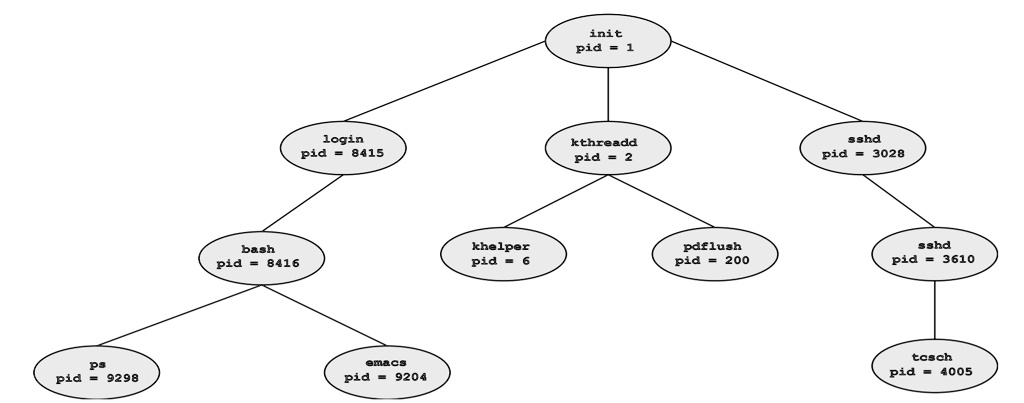
\includegraphics{process-tree}
  \caption{Example of a process tree}
  \labfig{process-tree}
\end{figure}

\subsection{Process Creation}
In linux systems, processes are managed by the kernel.
The kernel is responsible for creating, scheduling, and destroying processes.
The user can interact with the kernel using system calls to create, manage, and destroy processes.
Creating processes is simple, and can be done using the \textbf{fork()} system call.
This is used when any process wants to create a new process.

To simply create a new process for a command,
we can simply type in the command and press enter.
This will not only fork a new process from the terminal or
terminal emulator as the parent process, but also tie the
standard input, standard output, and standard error of the child process
to the terminal or terminal emulator.
\sidenote{
  Standard Input, Output, and Error are the default streams that are used by
  the shell to interact with the user. Standard Input is used to take input from
  the user, Standard Output is used to display output to the user, and Standard Error
  is used to display errors to the user. We will cover these in details in the next chapter.
}

\begin{lstlisting}[language=bash]
$ sleep 5
\end{lstlisting}

This will create a new process that will sleep for 5 seconds.

Remember that each process has a unique process id (PID).
Each process also has a parent process id (PPID),
which is the PID of the parent process.
If a process is created by the shell, the shell will be the parent process.
If the shell's process is killed, the child process will also
be killed, as the child process is owned by the shell.

\subsection{Process Ownership}

If you are using a linux operating system with a GUI server (X or Wayland),
try the following to understand how process ownership works.

Open two terminals, in the first one, run \lstinline|echo \$\$| to see the
process ID of that shell.
It should print out a random string of digits, that is the PID of the shell.
Then run a GUI application, such as \textbf{firefox}.
\sidenote{
  Make sure you are running something that is not running already.
}
This will block your terminal and open a new window of firefox.

\begin{lstlisting}[language=bash]
$ echo $$
2277503
$ firefox
\end{lstlisting}

Now in the other terminal, which is free, run \lstinline|pgrep firefox|
\sidenote{
  or whatever was your process's name
}
It should print out another random string of digits, it is the PID of
firefox.

Now you can use the following command to find the parent process's process
ID (PPID) to verify it is the same as the output of \lstinline|$$| in the first terminal.

\begin{lstlisting}[language=bash]
$ pgrep firefox
2278276
$ ps -efj | awk '$2==2278276;NR==1'
UID          PID    PPID    PGID     SID  C STIME TTY          TIME CMD
sayan    2278276 2277503 2278276 2277503 12 16:59 pts/5    00:00:03 /usr/lib/firefox/firefox
\end{lstlisting}

Here we can see that the PPID of firefox is the PID of the shell.

Note that the second command should put the PID of firefox, which we got
from the previous command. This can also be done in a single command
which you can directly copy and paste in your terminal.

\begin{lstlisting}[language=bash]
$ ps -efj | awk "\$2==$(pgrep firefox);NR==1"
UID          PID    PPID    PGID     SID  C STIME TTY          TIME CMD
sayan    2278276 2277503 2278276 2277503  1 16:59 pts/5    00:00:04 /usr/lib/firefox/firefox
\end{lstlisting}

Now, what happens if we kill the parent process?
To kill a process all we need to use is use the \lstinline|kill|
command with the PID of the process.

\begin{lstlisting}[language=bash]
$ kill -9 2277503
\end{lstlisting}

\marginnote{
  The \lstinline|-9| flag is used to send a \textbf{SIGKILL} signal to the process.
  This signal is used to kill a process immediately.
  We will cover signals later.
}

If you have been following along, you will see that both the terminal and firefox
dissapear from your screen. You will also notice that if you run the same
command to print the PID and PPID of firefox, it does not show anything.
This is because the process is killed and the process tree is destroyed, so
even firefox, being the child of the shell process, is killed.

\subsection{Don't kill my children}

However, there are also ways to create a new process in the background.
The easiest way to do this is to append an ampersand (\lstinline|&|) to the
end of the command. This is a shell syntax that tells the shell to fork the
command as a child process and run it in the background. What this means is
the shell will not wait for the command to finish, and will return the prompt
to the user immediately. However, the standard output and standard error may
still be tied to the terminal or terminal emulator. So if the process writes
something to the standard output or standard error, it will be displayed on the
terminal. Furthermore, the process is still owned by the shell, and if the shell
is killed, the process's parent will be changed to the \textbf{init} process.

Lets try the same exercise as earlier, but now with the \lstinline|&| at the end.

Open two terminals, and in the first one, execute the following command.

\begin{lstlisting}[language=bash]
$ echo $$
2400520
$ firefox &
[1] 2401297
$ echo "hello"
hello
$
ATTENTION: default value of option mesa_glthread overridden by environment.
$
\end{lstlisting}

You can observe that the firefox window opens up similar to last time, but
now the prompt returns immediately. You can also see that the output of the
\lstinline|echo| command is displayed on the terminal.

If you try to perform some operations in the browser, it may also print
some messages to the terminal screen, even though it is not waiting for
the command to finish. The "ATTENTION" message is an example of this.

Also observe that as soon as we launched \textbf{firefox}, it printed out
two numbers, [1] and 2401297. The number in the square brackets is the job
id of the process, and the number after that is the PID of the process.
So now we dont even need to use \lstinline|pgrep| to find the PID of the process.

Now in the other terminal, run the following command.

\begin{lstlisting}[language=bash]
$ ps -efj | awk "\$2==$(pgrep firefox);NR==1"
UID          PID    PPID    PGID     SID  C STIME TTY          TIME CMD
sayan    2401297 2400520 2401297 2400520  3 17:13 pts/5    00:00:08 /usr/lib/firefox/firefox
\end{lstlisting}

Still we can see that the PPID of firefox is the PID of the shell.

Now, if we kill the parent process, the child process will be adopted by the
init process, and will continue to run.

\begin{lstlisting}[language=bash]
$ kill -9 2400520
\end{lstlisting}

If you re-run the command to print the PID and PPID of firefox, you will see
that the PPID of firefox is now set to $1$, which is the PID of the \textbf{init}
command.

\begin{lstlisting}[language=bash]
$ ps -efj | awk "\$2==$(pgrep firefox);NR==1"
UID          PID    PPID    PGID     SID  C STIME TTY          TIME CMD
sayan    2401297       1 2401297 2400520  3 17:13 ?        00:00:09 /usr/lib/firefox/firefox
\end{lstlisting}

You can also see that the TTY column is now set to \lstinline|?|, which means that
the process is no longer tied to the terminal.

However, if instead of killing the parent process using the \textbf{SIGKILL}
signal, if you sent the \textbf{SIGHUP} signal to the parent, the child process
will still be terminated, as it will propagate the hangup signal to the child process.


\subsection{Setsid}

So how do we start a process directly in a way that it is not tied to the terminal?
Many times we would require to start a process in the background to run
asynchronously, but not always do we want to see the output of the process
in the terminal from where we launched it. We may also want the process
to be owned by the \textbf{init} process from the get go.

To do this, we can use the \lstinline|setsid| command. This command is used to
run a command in a new session. This will create a new process group and
set the PPID of the process to the \textbf{init} process. The TTY will also
be set to \lstinline|?|.

Lets try the same exercise with the \lstinline|setsid| command.
Open two terminals, in one of them, run the following command.

\begin{lstlisting}[language=bash]
$ echo $$
2453741
$ setsid -f firefox
$
\end{lstlisting}

Observe that firefox will open up, but the prompt will return immediately.

In another terminal, run the following command.

\begin{lstlisting}[language=bash]
$ ps -efj | awk "\$2==$(pgrep firefox);NR==1"
UID          PID    PPID    PGID     SID  C STIME TTY          TIME CMD
sayan    2454452       1 2454452 2454452  2 17:19 ?        00:00:07 /usr/lib/firefox/firefox
\end{lstlisting}

Observe that even without killing the parent process, the PPID of firefox is
already set to $1$, which is the PID of the \textbf{init} process.
So the process will not be killed if the shell is killed.

This is called a hang-up signal. We can still artificially send the
\textbf{SIGHUP} signal, which tells firefox that its parent has stopped
by using the \lstinline|kill -1| command.

\begin{lstlisting}[language=bash]
$ kill -1 2454452
\end{lstlisting}

This will still close firefox, even though the parent process (\textbf{init})
didn't actually get killed.

\subsection{Nohup}

If you do not want to give up the ownership of a child process,
and also don't really need to get the prompt back, but you do not
want to see the output of the command in your terminal. You can
use the \lstinline|nohup| command followed by the command you want to
run. It will still be tied to the terminal, and you can use
\lstinline|Ctrl+C| to stop it, \lstinline|Ctrl+Z| to pause it, etc.
The prompt will also be blocked till the process runs.
However, the input given to the terminal will not be sent
to the process, and the output of the process will not be
shown on the terminal. Instead, the output will be saved
in a file named \lstinline|nohup.out| in the current directory.

However, this is different from simply running the command
with a redirection operator (\lstinline|>|) at the end,
\sidenote{
  We will cover redirection operators in the next chapter.
}
because the \lstinline|nohup| command also makes the process
immune to the hang-up signal.

\begin{exercise}
  Try the same exercise as before, but this time use the \lstinline|nohup|
  to run firefox, then in another terminal, find the PID and PPID of
  firefox. Then try to kill the parent process and see if firefox
  dies or not.
\end{exercise}

\subsection{coproc}

The \lstinline|coproc| command is used to run a command in the background
and tie the standard input and standard output of the command to a
file descriptor. This is useful when you want to run a command in the
background, but still want to interact with it using the shell.
This creates a two way pipe between the shell and the command.

\textbf{Syntax}

\begin{lstlisting}[language=bash]
$ coproc [NAME] command [redirections]
\end{lstlisting}

This creates a coprocess named \lstinline|NAME| and runs the command in the background.
If the \lstinline|NAME| is not provided, the default name is \lstinline|COPROC|.

However, the recommended way to use \lstinline|coproc| is to use it in a
subshell, so that the file descriptors are automatically closed when
the subshell exits.

\begin{lstlisting}[language=bash]
$ coproc [NAME] { command; }
\end{lstlisting}

coproc can execute simple commands or compound commands. For simple
commands, name is not possible to be specified. Compound commands like
loops or conditionals can be executed using coproc in a subshell.

The name that is set becomes a array variable in the shell, and can be used
to access the file descriptors for stdin, stdout, and stderr.

For example, to provide input to the command, you can use \lstinline|echo| and
redirection operators to write to the file descriptor.

Similarly you can use the \lstinline|read| command to read from the file descriptor.

\begin{lstlisting}[language=bash]
$ coproc BC { bc -l; }
$ jobs
[1]+  Running                 coproc BC { bc -l; } &
$ echo 22/7 >&"${BC[1]}"
$ read output <&"${BC[0]}"
$ echo $output
3.14285714285714285714
\end{lstlisting}

This uses concepts from redirection and shell variables, which we will cover
in later weeks.

\subsection{at and cron}

Processes can also be scheduled to be launched at a later time.
This is usually done using \textbf{cron} or the \textbf{at} command.
We will cover these in depth later.

\subsection{GNU parallel}

GNU parallel is a shell tool for executing jobs in parallel using one
or more computers. A job can be a single command or a small script that
has to be run for each of the lines in the input. The typical input is
a list of files, a list of hosts, a list of users, a list of URLs, or a
list of tables. A job can also be a command that reads from a pipe.
GNU parallel can then split the input into blocks and pipe a block
into each command in parallel.

\subsection{systemd services}

Finally, the best way to run a background process or a daemon is to use
\textbf{systemd} services. \textbf{systemd} is an init system that is
used by most modern linux distributions. You can create a service file
declaring the process, the command line arguments, the environment variables,
and the user and group that the process should run as. You can also
specify if the process should be restarted if it crashes, or if it should
be started at boot time.


\vfill
\pagebreak
\section{Process Management}
\subsection{Disown}

Disown is a shell builtin command that is used to remove a job from the shell's
job table. This is useful when you have started a process in the background
and you want to remove it from the shell's job table, so that it is not
killed when the shell is killed. What it means is that if the parent
process recieves a hang-up signal, it will not propagate it to the child
job if it is removed from the job table.
This is applicable only for processes started from a shell.

Open two terminals, in one, open firefox in background using the \lstinline|&|

\begin{lstlisting}[language=bash]
$ firefox &
$
\end{lstlisting}

and then in the other terminal, run the following command.

\begin{lstlisting}[language=bash]
$ ps -efj | awk "\$2==$(pgrep firefox);NR==1"
UID          PID    PPID    PGID     SID  C STIME TTY          TIME CMD
sayan    3216429 3215856 3216429 3215856 69 18:45 pts/5    00:00:02 /usr/lib/firefox/firefox
$ kill -1 3215856
\end{lstlisting}

Observe that firefox will close, even though it was running in the background.
This is because the shell will propagate the hang-up signal to the child process.
If the parent shell was forcefully killed using the \textbf{SIGKILL} signal,
then it wont have the opportunity to propagate the hang-up signal to the child process.
This is a separate process than the natural killing of firefox running in
foreground even when shell is killed with \textbf{SIGKILL} signal.

Now, to fix this, we can simply run the \lstinline|disown| command in the terminal
where we started the firefox process.

Again open a terminal emulator and run the following command.

\begin{lstlisting}[language=bash]
$ firefox &
$ disown
$
\end{lstlisting}

Now, in the other terminal, run the following command.

\begin{lstlisting}[language=bash]
$ ps -efj | awk "\$2==$(pgrep firefox);NR==1"
UID          PID    PPID    PGID     SID  C STIME TTY          TIME CMD
sayan    3216429 3215856 3216429 3215856 69 18:45 pts/5    00:00:02 /usr/lib/firefox/firefox
$ kill -1 3215856
$ ps -efj | awk "\$2==$(pgrep firefox);NR==1"
UID          PID    PPID    PGID     SID  C STIME TTY          TIME CMD
sayan    3216429       1 3216429 3215856 10 18:45 ?        00:00:03 /usr/lib/firefox/firefox
\end{lstlisting}

Firefox does not close anymore, even when the parent process is hanged up.

\subsection{Jobs}

To list the jobs that are running in a shell, you can use the \lstinline|jobs| command.

\begin{lstlisting}[language=bash]
$ firefox &
$ sleep 50 &
$ jobs
[1]-  Running                 firefox &
[2]+  Running                 sleep 50 &
\end{lstlisting}

Here \lstinline|+| denotes the current job, and \lstinline|-| denotes the previous job.
The first column is the job number, it can also be used to refer to the job
inside that same shell. The process ID of a process can be used to refer to
the process from anywhere, but the job ID is only valid in the shell where
it is created.

The process id can be listed using the \lstinline|jobs -l| command.

\begin{lstlisting}[language=bash]
$ jobs -l
[1]- 3303198 Running                 firefox &
[2]+ 3304382 Running                 sleep 50 &
\end{lstlisting}

Using disown removes the job from this table. We can selectively
remove only some jobs from the table as well.

\begin{lstlisting}[language=bash]
$ jobs
[1]-  Running                 firefox &
[2]+  Running                 sleep 50 &
disown %1
$ jobs
[2]+  Running                 sleep 50 &
\end{lstlisting}

Whereas using \lstinline|disown -a| will remove all jobs from the table.
\lstinline|disown -r| will remove only running jobs from the table.

If you dont really want to lose the job from the table, but you want to
prevent it from being killed when the shell is killed, you can use
\lstinline|disown -h| to mark the jobs to be ignored by the hang-up signal.
It will have same effect as last exercise, but it will still be present
in the output of the \lstinline|jobs| command.

\subsection{Suspending and Resuming Jobs}

Sometimes you may want to pause a job and resume it later.
This is supported directly by the linux kernel.
To pause any process you can send it the \textbf{SIGSTOP} or \textbf{SIGTSTP} signal.
\sidenote{
  The difference between \textbf{SIGSTOP} and \textbf{SIGTSTP} is that
  \textbf{SIGSTOP} is a signal that cannot be caught or ignored by the process,
  so the process will be paused immediately. \textbf{SIGTSTP} is a signal that
  can be caught or ignored by the process, so the process can do some cleanup
  before pausing. The default action of \textbf{SIGTSTP} is to pause the process.
}
This can be done using the same \textbf{kill} command. The signal number for
\textbf{SIGSTOP} is 19, and for \textbf{SIGTSTP} is 20.

To resume the process, you can send it the \textbf{SIGCONT} signal.
The signal number for \textbf{SIGCONT} is 18.

\begin{exercise}
  Try to pause a job using the \textbf{SIGSTOP} signal, then resume it using the
  \textbf{SIGCONT} signal.
  Open firefox from a terminal using \lstinline|firefox \&| and note the PID,
  then pause it using
  \lstinline|kill -19 <PID>|,
  try to click on the firefox window, and see if it responds.
  Then resume it using \lstinline|kill -18 <PID>|.
  Does the firefox window respond now?
\end{exercise}

If you start a command from the shell without using the \lstinline|&| operator,
you can pause the command using \lstinline|Ctrl+Z| and resume it using the
\lstinline|fg| command.
This sends the same signals as above, and uses the shell's job table
to keep track of the jobs.

\begin{remark}
  Just like disown, the \lstinline|fg| command can also take the job number
  as an argument to bring that job to the foreground. The default job
  is the current job. (Marked with a \lstinline|+| in the \lstinline|jobs| command))
\end{remark}

You can also use the \lstinline|bg| command to resume a job, but in the background.
This has same effect as using the \lstinline|&| operator at the end of the command.

\begin{remark}
  Since the disown, fg, and bg commands work on the shell's job table,
  they are shell builtins, and not a executable binary.
  You can verify this using the \lstinline|type| command.
\end{remark}

You cannot perform job control on a process that is not started from the shell,
or if you have disowned the process.

\subsection{Killing Processes}

We have been using the \lstinline|kill| command to send signals to processes.
The kill command is a shell builtin and an executable command that is used
to send signals to processes. The default signal that is sent is the
\textbf{SIGTERM} signal, which is signal number 15.
The kill command is the user-land way to communicate with the kernel that
some process needs to be given a certain signal.

\textbf{Syntax}

\begin{lstlisting}[language=bash]
$ kill [-signal|-s signal] PID|name...
\end{lstlisting}

Let us also briefly discuss what the synopsis of the command means, and
how to interpret it.

The first word is the name of the command, which is \lstinline|kill| in this case.
The argument \textbf{signal} inside square brackets means that it is optional.
The argument \textbf{PID} is the process ID of the process that you want to kill.
The argument \textbf{name} is the name of the process that you want to kill.
The pipe between \textbf{PID} and \textbf{name} means that you can provide
either the PID or the name of the process.
The ellipsis (\lstinline|...|) after \textbf{PID|name} means that you can provide
as many PIDs or names as you want.

\begin{remark}
  As mentioned, kill is also a shell builtin command. This means that
  the synopsis seen in the man page of kill is not the same as the
  synopsis of the builtin. The bash builtin of kill does not support
  providing names of the processes, only the PIDs. Hence if you want
  to kill a process by its name, you will either have to use the
  path of the kill binary, or use the \lstinline|pkill| command.
\end{remark}

So for example, we can run kill in the following manners.

\begin{lstlisting}[language=bash]
$ kill 2452
$ kill -9 2452
$ kill -9 2452 62
$ kill -SIGKILL 2525
$ kill -SIGKILL 2525 732
\end{lstlisting}

The \lstinline|kill| command can also be used to send other non-terminating signals
to the process. For example, the \textbf{SIGSTP} signal can be used to pause
a process, and the \textbf{SIGCONT} signal can be used to resume a process.
Similarly, there are some undefined signals that can be used to send custom
signals to the process.

\textbf{SIGUSR1} and \textbf{SIGUSR2} are signals that do not have any predefined
behaviour, and can be used by the user to send custom signals to the process.
The behaviour of the process on receipt of these signals is decided by the
process and told to the user by the process documentation. The user can
then send these signals to the process using the \lstinline|kill| command.
This helps user interact with processes that are not running directly in the
foreground of a shell.

Processes can also \textbf{trap} signals, which means that they can catch
a signal and run a custom handler function. This is useful when you want
to do some cleanup before the process is killed. This can also be used
to totally change how the process behaves on receipt of a signal.
However, to prevent malicious code from running, the \textbf{SIGKILL} signal
cannot be trapped, and the process will be killed immediately. Similarly
the \textbf{SIGSTOP} signal, which is similar in definition to the \textbf{SIGSTP}
signal, cannot be trapped.

To see the list of the signals, we can run \lstinline|kill -l|.

\begin{lstlisting}[language=bash]
$ kill -l
 1) SIGHUP       2) SIGINT       3) SIGQUIT      4) SIGILL       5) SIGTRAP
 6) SIGABRT      7) SIGBUS       8) SIGFPE       9) SIGKILL     10) SIGUSR1
11) SIGSEGV     12) SIGUSR2     13) SIGPIPE     14) SIGALRM     15) SIGTERM
16) SIGSTKFLT   17) SIGCHLD     18) SIGCONT     19) SIGSTOP     20) SIGTSTP
21) SIGTTIN     22) SIGTTOU     23) SIGURG      24) SIGXCPU     25) SIGXFSZ
26) SIGVTALRM   27) SIGPROF     28) SIGWINCH    29) SIGIO       30) SIGPWR
31) SIGSYS      34) SIGRTMIN    35) SIGRTMIN+1  36) SIGRTMIN+2  37) SIGRTMIN+3
38) SIGRTMIN+4  39) SIGRTMIN+5  40) SIGRTMIN+6  41) SIGRTMIN+7  42) SIGRTMIN+8
43) SIGRTMIN+9  44) SIGRTMIN+10 45) SIGRTMIN+11 46) SIGRTMIN+12 47) SIGRTMIN+13
48) SIGRTMIN+14 49) SIGRTMIN+15 50) SIGRTMAX-14 51) SIGRTMAX-13 52) SIGRTMAX-12
53) SIGRTMAX-11 54) SIGRTMAX-10 55) SIGRTMAX-9  56) SIGRTMAX-8  57) SIGRTMAX-7
58) SIGRTMAX-6  59) SIGRTMAX-5  60) SIGRTMAX-4  61) SIGRTMAX-3  62) SIGRTMAX-2
\end{lstlisting}

Some of the important signals are:

\begin{itemize}
  \item \textbf{SIGHUP} - Hangup signal. This is sent to a process when the
  terminal is closed. This is used to tell the process that the terminal
  is no longer available.
\item \textbf{SIGINT} - Interrupt signal. This is sent to a process when the
  user presses \lstinline|Ctrl+C|. This is used to tell the process to stop
  what it is doing and exit.
\item \textbf{SIGKILL} - Kill signal. This is used to kill a process immediately.
  This signal cannot be caught or ignored by the process.
\item \textbf{SIGTERM} - Terminate signal. This is used to tell the process
  to exit gracefully. The process can catch this signal and do some cleanup
  before exiting. This is the default signal sent by the \lstinline|kill| command.
\item \textbf{SIGSTP} - Stop signal. This is used to pause a process.
  This is sent when the user presses \lstinline|Ctrl+Z|. This signal can be
  caught or ignored by the process.
\item \textbf{SIGSTOP} - Stop signal. This is used to pause a process.
  This signal cannot be caught or ignored by the process.
\item \textbf{SIGCONT} - Continue signal. This is used to resume a process
  that has been paused using the \textbf{SIGSTOP} signal. This is sent
  when the user presses \lstinline|fg| or \lstinline|bg|.
\item \textbf{SIGUSR1} - User defined signal 1. This is a signal that can
  be used by the user to send a custom signal to the process.
\item \textbf{SIGUSR2} - User defined signal 2. This is a signal that can
  be used by the user to send a custom signal to the process.
\item \textbf{SIGCHLD} - Child signal. This is sent to the parent process
  when a child process exits. This is used to tell the parent process that
  the child process has exited.
\item \textbf{SIGSEGV} - Segmentation fault signal. This is sent to a process
  when it tries to access memory that it is not allowed to access.
\item \textbf{SIGPIPE} - Pipe signal. This is sent to a process when it tries
  to write to a pipe that has been closed.
\end{itemize}

\vfill
\pagebreak
\section{Finding Processes}

As we saw, managing a process is easy once we know the PID of the process.
However, it is not always easy to find the PID of a process.
To do this, there are multiple tools in linux that can be used.

\subsection{pgrep}

The \lstinline|pgrep| command is used to find the PID of a process based on its name.
It can take the name of the process as an argument, and will print the PID of the
processes that match the name. The search can also be a regex pattern.
\sidenote{
  We will discuss regex patterns in the next chapter.
}
We have already seen how \lstinline|pgrep| can be used to find the PID of a process.

\begin{lstlisting}[language=bash]
$ pgrep firefox
526272
\end{lstlisting}

We can also use it for any process run from the terminal.

\begin{lstlisting}[language=bash]
$ sleep 50 &
$ sleep 20 &
$ sleep 10 &
$ pgrep sleep
98963
99332
99526
\end{lstlisting}

\subsection{pkill}

Similarly, we also have the \lstinline|pkill| command, which is used to kill a process
based on its name. It can take the name of the process as an argument, and will
send the \textbf{SIGTERM} signal to the processes that match the name.
Other signals can also be sent using the \lstinline|-signal| flag, similar to the
kill command.

\begin{lstlisting}[language=bash]
$ pkill firefox
\end{lstlisting}

\subsection{pidwait}

The \lstinline|pidwait| command is used to wait for a process to exit.
It searches for the process using its name, a part of its name, or any
regex matching its name, and waits for the process to exit.

\begin{exercise}
  Open firefox from a terminal in the background, then use the \lstinline|pidwait|
  to wait till the process exits. After some time, close the firefox window
  and observe the terminal.
\end{exercise}

\vfill
\pagebreak
\section{Listing Processes}

Sometimes we may not even know the name of the process, and we may want to
list all the processes running on the system. This can be done using the
many commands.

\subsection{ps}

\textbf{ps} is an ancient command
\sidenote{
  It exists in the Unix V7 manual, which was released in 1979.
  It has BSD-like options, GNU-like options, and System V-like options.
}
that is used to list the processes running on the system.

There are a lot of options and flags that can be used with the \textbf{ps} command.
The flags are of multiple types, and some flags perform the same function but
are named differently. This is because the \textbf{ps} command has been around
for a long time, and has been implemented in multiple ways in different systems.
There are also different formats in which the output can be displayed.

The most common flags used with the \textbf{ps} command are:

\begin{itemize}
  \item \textbf{ps} - This will get a snapshot of the processes owned by the user tied to the TTY.
  \item \textbf{ps -e} - This will show all the processes.
  \item \textbf{ps -f} - This will show full format listing.
  \item \textbf{ps -l} - This will show long format listing.
  \item \textbf{ps u} - This will show user-oriented format listing.
  \item \textbf{ps x} - This will show processes without controlling terminals.
  \item \textbf{ps -A} - This will show all processes.
  \item \textbf{ps aux} - This is a common command to see all processes owned by all users with and without TTY associations and showing the user who owns them.
  \item \textbf{ps --forest} - This will show the processes in a tree form.
\end{itemize}

There are hundreds of flags that can be used with the \textbf{ps} command.

\begin{exercise}
  Try to use the \textbf{ps} command with the flags mentioned above, and see
  the output of the command.
\end{exercise}

\subsection{pstree}

The \textbf{pstree} command is used to display the processes in a tree form.
Although the \textbf{ps} command can also display the processes in a tree form
using the \lstinline|--forest| flag, the \textbf{pstree} command is more suited
for this purpose. It has many features that ps lacks, such as collapsing
branches of identical processes, better ASCII art, Unicode support, etc.

If the system and the terminal supports unicode, the \textbf{pstree} command
will automatically use
\href{https://en.wikipedia.org/wiki/Box-drawing\_character}{VT100 box-drawing characters}
to make the tree look better. We can still force it to use ASCII with the
\lstinline|-A| flag.

We can also disable the clubbing of identical processes using the \lstinline|-c| flag.

The pstree command optionally takes a PID as an argument, and will display
the tree rooted at that PID. If no PID is provided, it will display the
tree rooted at the init process.

I can find the PID of the tmux server I am running to develop this book
using the \lstinline|pgrep| command.
\begin{lstlisting}[language=bash]
$ pgrep tmux
62957
\end{lstlisting}

And then use the \lstinline|pstree| command
to display the tree rooted at that PID.

\begin{lstlisting}[language=bash]
$ pstree -A 62957
tmux: server-+-bash---nvim-+-nvim-+-node---14*[{node}]
             |             |      |-texlab---9*[{texlab}]
             |             |      |-xsel
             |             |      `-9*[{nvim}]
             |             `-2*[{nvim}]
             |-bash---watch.sh---entr
             |-bash---zathura---8*[{zathura}]
             |-3*[bash]
             |-2*[bash---man---less]
             |-bash---nvim-+-nvim-+-2*[node---9*[{node}]]
             |             |      `-{nvim}
             |             `-2*[{nvim}]
             `-bash-+-pstree
                    `-xsel
\end{lstlisting}

This helps us easily find out which processes are running under which process,
and helps us understand the process tree.

\subsection{top}

The \textbf{top} command is used to display the processes that are running
in real time. It is an interactive command that displays the processes in
a table format, and updates the table every few seconds. It also displays
the CPU and memory usage of the processes.

The \textbf{top} command is very useful when you want to monitor the processes
and the resources they are using in real time. It is also useful when you
want to find out which process is using the most CPU or memory.

Since it is an interactive command, it has keyboard shortcuts as well, along
with runtime options that can be used to change the behaviour of the command.

\marginnote{
  Note: The output of the \textbf{top} command is not static, and it contains
  control characters and
  \href{https://en.wikipedia.org/wiki/ANSI\_escape\_code}{ANSI escape codes}
  to make the output beautiful and interactive. This is why the output is not
  suitable for use in scripts, and is only meant for human consumption.
  I have removed the control characters and ANSI escape codes from the output
  shown here.
}

\begin{lstlisting}
$ top
top - 15:44:55 up 40 min,  1 user,  load average: 2.03, 1.37, 1.02
Tasks: 271 total,   1 running, 270 sleeping,   0 stopped,   0 zombie
%Cpu(s):  9.8 us,  4.9 sy,  0.0 ni, 85.4 id,  0.0 wa,  0.0 hi,  0.0 si,  0.0 st
MiB Mem :   7764.2 total,    604.5 free,   5663.2 used,   1919.6 buff/cache
MiB Swap:  20002.0 total,  19901.2 free,    100.8 used.   2101.0 avail Mem

    PID USER      PR  NI    VIRT    RES    SHR S  %CPU  %MEM     TIME+ COMMAND
    631 sayan     20   0 1248084  81976  44580 S  18.2   1.0   1:39.82 Xorg
   1072 sayan     20   0 3159356 229336  89816 S   9.1   2.9   0:44.01 spotify
   1079 sayan     20   0 1123.5g 128252  65776 S   9.1   1.6   0:09.37 Discord
      1 root      20   0   22076  12840   9476 S   0.0   0.2   0:03.62 systemd
      2 root      20   0       0      0      0 S   0.0   0.0   0:00.00 kthreadd
      3 root      20   0       0      0      0 S   0.0   0.0   0:00.00 pool_wo+
\end{lstlisting}

\subsection{htop}

The \textbf{htop} command is an interactive process viewer for Unix systems.
It is inspired from the \textbf{top} command, but has a lot more features
such as scrolling the process list, searching for processes, killing processes,
tree view of processes, etc.

\begin{exercise}
  Run (Install if not present) the \textbf{htop} command and see the output.
  Notice how the output is more interactive and colourful than the \textbf{top}
  command. Run something heavy in the background, and see how the CPU and
  the memory usage changes in real time.
\end{exercise}

One such command to run to simulate heavy CPU usage is to run the following command.

\begin{lstlisting}[language=bash]
$ cat /dev/urandom | gzip > /dev/null &
\end{lstlisting}

This will compress the random data from \lstinline|/dev/urandom| and write it to
\lstinline|/dev/null|. This will use a lot of CPU, and you can see the CPU usage
spike up. But this is a single core process, so the CPU usage will be limited
to only one core. However, the CPU core used may keep changing.

\begin{remark}
  The above command is a simple way to generate CPU usage. It will not
  write any data to disk and not eat any disk space. However, the
  command should be typed carefully, since if you forget to add the
  \lstinline|> /dev/null| part, it will write the compressed data to the
  terminal if \lstinline|-f| is given to \lstinline|gzip|, and the terminal
  will be filled with random data and get messed up. In this case
  you can type \lstinline|tput reset| to reset the terminal after killing
  the process.
\end{remark}

\subsection{btop}

The \textbf{btop} command is a terminal based graphical process viewer.
It is inspired from the \textbf{htop} command, but has a more graphical
interface. It is written in python, and uses the \textbf{blessings} library
to draw the interface.

\subsection{glances}

The \textbf{glances} command is a cross-platform monitoring tool that is
used to monitor the system resources in real time. It is written in python,
and uses the \textbf{curses} library to draw the interface.


\vfill
\pagebreak
\section{Exit Codes}

Every process that runs in linux has an exit code when it terminates.
This is a number that is returned by the process to the parent process
when it exits. This number is used to tell the parent process if the
process exited successfully or not. The exit code is a number between
0 and 255, and is used to tell the parent process the status of the
child process.

The exit code of the last run process is stored in a variable
called \lstinline|$?| in the shell. Successful processes return 0,
whereas unsuccessful processes return a non-zero number.
The exact return code is decided by the process itself, and usually
has some meaning to the process. Some common exit codes are:

\begin{itemize}
  \item 0 - Success
  \item 1 - General error
  \item 2 - Misuse of shell builtins
  \item 126 - Command invoked cannot execute
  \item 127 - Command not found
  \item 128 - Invalid argument to exit
  \item 128+n - Fatal error signal "n"
  \item 130 - Script terminated by \lstinline|Ctrl+C|
  \item 137 - Process killed with \textbf{SIGKILL}
  \item 255 - Exit status out of range
\end{itemize}

\begin{remark}
Note that $130=128+2$, and $2$ is the signal number for \textbf{SIGINT},
thus, the exit code for a process that is terminated by \lstinline|Ctrl+C|
is 130. Similarly, any other signal sent to the process causing it to
exit abnormally will have an exit code of $128+n$, where $n$ is the signal
number. Similarly $137=128+9$, and $9$ is the signal number for \textbf{SIGKILL}.
\end{remark}

To return any exit status from your script, you can use the \lstinline|exit| command.

\begin{lstlisting}[language=bash]
$ cat myscript.sh
#!/bin/bash
echo "hello"
exit 25
$ ./script.sh
bash: ./script.sh: No such file or directory
$ echo $?
127
$ ./myscript.sh
bash: ./myscript.sh: Permission denied
$ echo $?
126
$ chmod u+x myscript.sh
$ ./myscript.sh
hello
$ echo $?
25
\end{lstlisting}

The exit code is how shell constructs like \lstinline|if|, \lstinline|while|,
and \lstinline|until| construct their conditions. If the exit code is 0,
then it is considered true, and if the exit code is non-zero, then it
is considered false.

\begin{lstlisting}[language=bash]
$ if ./myscript.sh; then echo "success"; else echo "failure $?"; fi
hello
failure 25
$ if ls /bin/bash; then echo "success"; else echo "failure $?"; fi
/bin/bash
success
\end{lstlisting}


\appendix % From here onwards, chapters are numbered with letters, as is the appendix convention

\pagelayout{wide} % No margins
\addpart{Appendix}
\pagelayout{margin} % Restore margins

% \input{chapters/appendix.tex}

%----------------------------------------------------------------------------------------

\backmatter % Denotes the end of the main document content
\setchapterstyle{plain} % Output plain chapters from this point onwards

%----------------------------------------------------------------------------------------
%	BIBLIOGRAPHY
%----------------------------------------------------------------------------------------

% The bibliography needs to be compiled with biber using your LaTeX editor, or on the command line with 'biber main' from the template directory

\defbibnote{bibnote}{Here are the references in citation order.\par\bigskip} % Prepend this text to the bibliography
\printbibliography[heading=bibintoc, title=Bibliography, prenote=bibnote] % Add the bibliography heading to the ToC, set the title of the bibliography and output the bibliography note

%----------------------------------------------------------------------------------------
%	NOMENCLATURE
%----------------------------------------------------------------------------------------

% The nomenclature needs to be compiled on the command line with 'makeindex main.nlo -s nomencl.ist -o main.nls' from the template directory

\nomenclature{$c$}{Speed of light in a vacuum inertial frame}
\nomenclature{$h$}{Planck constant}

\renewcommand{\nomname}{Notation} % Rename the default 'Nomenclature'
\renewcommand{\nompreamble}{The next list describes several symbols that will be later used within the body of the document.} % Prepend this text to the nomenclature

\printnomenclature % Output the nomenclature

%----------------------------------------------------------------------------------------
%	GREEK ALPHABET
% 	Originally from https://gitlab.com/jim.hefferon/linear-algebra
%----------------------------------------------------------------------------------------

\vspace{1cm}

{\usekomafont{chapter}Greek Letters with Pronunciations} \\[2ex]
\begin{center}
	\newcommand{\pronounced}[1]{\hspace*{.2em}\small\textit{#1}}
	\begin{tabular}{l l @{\hspace*{3em}} l l}
		\toprule
		Character & Name & Character & Name \\
		\midrule
		$\alpha$ & alpha \pronounced{AL-fuh} & $\nu$ & nu \pronounced{NEW} \\
		$\beta$ & beta \pronounced{BAY-tuh} & $\xi$, $\Xi$ & xi \pronounced{KSIGH} \\
		$\gamma$, $\Gamma$ & gamma \pronounced{GAM-muh} & o & omicron \pronounced{OM-uh-CRON} \\
		$\delta$, $\Delta$ & delta \pronounced{DEL-tuh} & $\pi$, $\Pi$ & pi \pronounced{PIE} \\
		$\epsilon$ & epsilon \pronounced{EP-suh-lon} & $\rho$ & rho \pronounced{ROW} \\
		$\zeta$ & zeta \pronounced{ZAY-tuh} & $\sigma$, $\Sigma$ & sigma \pronounced{SIG-muh} \\
		$\eta$ & eta \pronounced{AY-tuh} & $\tau$ & tau \pronounced{TOW (as in cow)} \\
		$\theta$, $\Theta$ & theta \pronounced{THAY-tuh} & $\upsilon$, $\Upsilon$ & upsilon \pronounced{OOP-suh-LON} \\
		$\iota$ & iota \pronounced{eye-OH-tuh} & $\phi$, $\Phi$ & phi \pronounced{FEE, or FI (as in hi)} \\
		$\kappa$ & kappa \pronounced{KAP-uh} & $\chi$ & chi \pronounced{KI (as in hi)} \\
		$\lambda$, $\Lambda$ & lambda \pronounced{LAM-duh} & $\psi$, $\Psi$ & psi \pronounced{SIGH, or PSIGH} \\
		$\mu$ & mu \pronounced{MEW} & $\omega$, $\Omega$ & omega \pronounced{oh-MAY-guh} \\
		\bottomrule
	\end{tabular} \\[1.5ex]
	Capitals shown are the ones that differ from Roman capitals.
\end{center}

%----------------------------------------------------------------------------------------
%	GLOSSARY
%----------------------------------------------------------------------------------------

% The glossary needs to be compiled on the command line with 'makeglossaries main' from the template directory

\setglossarystyle{listgroup} % Set the style of the glossary (see https://en.wikibooks.org/wiki/LaTeX/Glossary for a reference)
\printglossary[title=Special Terms, toctitle=List of Terms] % Output the glossary, 'title' is the chapter heading for the glossary, toctitle is the table of contents heading

%----------------------------------------------------------------------------------------
%	INDEX
%----------------------------------------------------------------------------------------

% The index needs to be compiled on the command line with 'makeindex main' from the template directory

\printindex % Output the index

%----------------------------------------------------------------------------------------
%	BACK COVER
%----------------------------------------------------------------------------------------

% If you have a PDF/image file that you want to use as a back cover, uncomment the following lines

%\clearpage
%\thispagestyle{empty}
%\null%
%\clearpage
%\includepdf{cover-back.pdf}

%----------------------------------------------------------------------------------------

\end{document}
